\documentclass[conference]{IEEEtran}
\IEEEoverridecommandlockouts
\usepackage{cite}
\usepackage{amsmath,amssymb,amsfonts}
\usepackage{algorithmic}
\usepackage{graphicx}
\usepackage{booktabs}
\usepackage{multirow}
\usepackage{xcolor}
\usepackage{textcomp}
\usepackage[hidelinks]{hyperref}
\usepackage{url}
\graphicspath{{figures/}}

% ---- numbers injected from experiments (with safe fallbacks) ----
\providecommand{\nTickers}{11}
\providecommand{\nObs}{10{,}704}
\providecommand{\nArticles}{18{,}600}
\providecommand{\newsCov}{34.7}
\providecommand{\dateMin}{2018}
\providecommand{\dateMax}{2023}
\providecommand{\RleakRand}{0.999}
\providecommand{\RleakChrono}{0.999}
\providecommand{\RleakPersist}{0.999}
\providecommand{\RleakReturns}{-0.037}
\providecommand{\vifClose}{22{,}977}
\providecommand{\vifStatMax}{1{,}347}
\providecommand{\shapSentShare}{X}
\providecommand{\igSentShare}{X}
\providecommand{\permSentShare}{X}
\providecommand{\blockPermSent}{X}
\providecommand{\blockPermPrice}{X}
\providecommand{\sentOnlyMaxMCC}{X}
\providecommand{\bestDirAcc}{X}
\providecommand{\majAcc}{X}
\providecommand{\sentDeltaAcc}{X}
\providecommand{\sentCIlo}{X}
\providecommand{\sentCIhi}{X}
\providecommand{\edaKurtosis}{X}
\providecommand{\edaCrossCorr}{X}
\providecommand{\edaAcfClose}{X}
\providecommand{\edaAcfReturn}{X}
\providecommand{\edaFeatTargetMax}{X}
\providecommand{\edaSentTargetMax}{X}
\providecommand{\edaLevelsNonstat}{X}
\providecommand{\edaReturnsStat}{X}
\providecommand{\edaUpRate}{X}
\providecommand{\nModelsZoo}{X}
\providecommand{\nModelsZooCiScored}{X}
\providecommand{\modelZooMaxMCC}{X}
\providecommand{\modelZooMeanAcc}{X}
\providecommand{\faithUniverseN}{X}
\providecommand{\faithRhoBar}{X}
\providecommand{\faithEffN}{X}
\providecommand{\nXaiMethodsCatalogued}{X}
\providecommand{\nXaiFaithfulOfScoreable}{X}
% R3 revision macros (M1/M2/M5/M6) -- generated per-method by make_tables.py;
% fallbacks here cover treeshap/kernelshap/lime/permutation.
\providecommand{\marginTreeshap}{X}\providecommand{\mdesTreeshap}{X}\providecommand{\mdesRatioTreeshap}{X}
\providecommand{\pctSymTreeshap}{X}\providecommand{\pctSymCiLoTreeshap}{X}\providecommand{\pctSymCiHiTreeshap}{X}
\providecommand{\marginKernelshap}{X}\providecommand{\mdesKernelshap}{X}\providecommand{\mdesRatioKernelshap}{X}
\providecommand{\pctSymKernelshap}{X}\providecommand{\pctSymCiLoKernelshap}{X}\providecommand{\pctSymCiHiKernelshap}{X}
\providecommand{\marginLime}{X}\providecommand{\mdesLime}{X}\providecommand{\mdesRatioLime}{X}
\providecommand{\pctSymLime}{X}\providecommand{\pctSymCiLoLime}{X}\providecommand{\pctSymCiHiLime}{X}
\providecommand{\marginPermutation}{X}\providecommand{\mdesPermutation}{X}\providecommand{\mdesRatioPermutation}{X}
\providecommand{\pctSymPermutation}{X}\providecommand{\pctSymCiLoPermutation}{X}\providecommand{\pctSymCiHiPermutation}{X}
\providecommand{\mcnemarPTreeshap}{X}\providecommand{\wilcoxonPTreeshap}{X}
\providecommand{\mcnemarPKernelshap}{X}\providecommand{\wilcoxonPKernelshap}{X}
\providecommand{\mcnemarPLime}{X}\providecommand{\wilcoxonPLime}{X}
\providecommand{\nWeakSignalScored}{X}
\providecommand{\nModelsZooCiScored}{X}
\providecommand{\nAgreementMethods}{X}\providecommand{\nAgreementExcluded}{X}
\providecommand{\agreementRhoMin}{X}\providecommand{\agreementRhoMax}{X}\providecommand{\agreementRhoMean}{X}
\providecommand{\nSensRuns}{X}\providecommand{\sensPctInterpMin}{X}\providecommand{\sensPctInterpMax}{X}
\providecommand{\sensPctInterpMean}{X}\providecommand{\nSensRunsWithNotable}{X}
\providecommand{\sensMaxZMin}{X}\providecommand{\sensMaxZMax}{X}\providecommand{\nSensDistinctTop}{X}
\providecommand{\sensMajorityComponent}{X}\providecommand{\sensMajorityN}{X}\providecommand{\sensTotalRuns}{X}
\renewcommand{\RleakRand}{0.999}
\renewcommand{\RleakChrono}{0.994}
\renewcommand{\RleakPersist}{1.000}
\renewcommand{\RleakReturns}{-0.033}
\renewcommand{\bestDirAcc}{51.3}
\renewcommand{\majAcc}{51.3}
\renewcommand{\sentDeltaAcc}{-0.13}
\renewcommand{\sentCIlo}{-0.39}
\renewcommand{\sentCIhi}{0.14}
\renewcommand{\shapSentShare}{8.0}
\renewcommand{\igSentShare}{32.6}
\renewcommand{\permSentShare}{0.0}
\renewcommand{\blockPermSent}{-0.28}
\renewcommand{\blockPermPrice}{-0.38}
\renewcommand{\sentOnlyMaxMCC}{0.028}
\renewcommand{\vifClose}{20,505}
\renewcommand{\vifStatMax}{5}
\renewcommand{\edaKurtosis}{17.3}
\renewcommand{\edaCrossCorr}{0.38}
\renewcommand{\edaAcfClose}{0.991}
\renewcommand{\edaAcfReturn}{-0.081}
\renewcommand{\edaFeatTargetMax}{0.051}
\renewcommand{\edaSentTargetMax}{0.005}
\renewcommand{\edaLevelsNonstat}{96}
\renewcommand{\edaReturnsStat}{100}
\renewcommand{\edaUpRate}{52.1}
\renewcommand{\nTickers}{57}
\renewcommand{\nObs}{127,609}
\renewcommand{\newsCov}{47.8}
\renewcommand{\dateMin}{2015}
\renewcommand{\dateMax}{2023}
\renewcommand{\nModelsZooCiScored}{3}
\renewcommand{\nModelsZoo}{16}
\renewcommand{\modelZooMaxMCC}{0.011}
\renewcommand{\modelZooMeanAcc}{0.506}
\renewcommand{\faithUniverseN}{57}
\renewcommand{\faithRhoBar}{0.381}
\renewcommand{\faithEffN}{2.55}
\renewcommand{\nWeakSignalScored}{4}
\renewcommand{\mdesRatioTreeshap}{22.4}
\renewcommand{\marginTreeshap}{0.146}
\renewcommand{\mdesTreeshap}{0.0065}
\renewcommand{\pctSymTreeshap}{100.0}
\renewcommand{\pctSymCiLoTreeshap}{100.0}
\renewcommand{\pctSymCiHiTreeshap}{100.0}
\renewcommand{\mdesRatioKernelshap}{17.1}
\renewcommand{\marginKernelshap}{0.034}
\renewcommand{\mdesKernelshap}{0.0020}
\renewcommand{\pctSymKernelshap}{100.0}
\renewcommand{\pctSymCiLoKernelshap}{100.0}
\renewcommand{\pctSymCiHiKernelshap}{100.0}
\renewcommand{\mdesRatioLime}{15.6}
\renewcommand{\marginLime}{0.058}
\renewcommand{\mdesLime}{0.0037}
\renewcommand{\pctSymLime}{100.0}
\renewcommand{\pctSymCiLoLime}{100.0}
\renewcommand{\pctSymCiHiLime}{100.0}
\renewcommand{\mdesRatioPermutation}{2.5}
\renewcommand{\marginPermutation}{0.021}
\renewcommand{\mdesPermutation}{0.0085}
\renewcommand{\pctSymPermutation}{78.9}
\renewcommand{\pctSymCiLoPermutation}{68.4}
\renewcommand{\pctSymCiHiPermutation}{89.5}
\renewcommand{\mcnemarPTreeshap}{$<$0.001}
\renewcommand{\wilcoxonPTreeshap}{$<$0.001}
\renewcommand{\mcnemarPKernelshap}{$<$0.001}
\renewcommand{\wilcoxonPKernelshap}{$<$0.001}
\renewcommand{\mcnemarPLime}{$<$0.001}
\renewcommand{\wilcoxonPLime}{$<$0.001}
\renewcommand{\nAgreementMethods}{4}
\renewcommand{\agreementRhoMin}{0.10}
\renewcommand{\agreementRhoMax}{0.93}
\renewcommand{\agreementRhoMean}{0.51}
\renewcommand{\nAgreementExcluded}{10}
\renewcommand{\nSensRuns}{6}
\renewcommand{\sensPctInterpMin}{98.8}
\renewcommand{\sensPctInterpMax}{100.0}
\renewcommand{\sensPctInterpMean}{99.2}
\renewcommand{\nSensRunsWithNotable}{6}
\renewcommand{\sensMaxZMin}{2.05}
\renewcommand{\sensMaxZMax}{2.81}
\renewcommand{\nSensDistinctTop}{2}
\renewcommand{\sensMajorityComponent}{layer1\_full}
\renewcommand{\sensMajorityN}{5}
\renewcommand{\sensTotalRuns}{6}
\renewcommand{\nXaiMethodsCatalogued}{23}
\renewcommand{\nXaiFaithfulOfScoreable}{16/16}
\renewcommand{\tcavPEmp}{1.00}
\renewcommand{\tcavNullMeanRange}{0.53--0.58}
\renewcommand{\saeNullMean}{0.00}
\renewcommand{\saeNullPHi}{0.00}
\renewcommand{\saeNullMax}{0}
\renewcommand{\ablNullMean}{1.00}
\renewcommand{\ablNullPHi}{1.00}
\renewcommand{\recurC}{10}
\renewcommand{\recurK}{5}
\renewcommand{\recurR}{6}
\renewcommand{\recurPBinomOne}{5.5\times10^{-5}}
\renewcommand{\recurPUnion}{5.5\times10^{-4}}
\renewcommand{\yearMarginMinTreeshap}{0.146}
\renewcommand{\yearMarginMaxTreeshap}{0.164}
\renewcommand{\yearCopyCreditMinTreeshap}{0.189}
\renewcommand{\yearCopyCreditMaxTreeshap}{0.221}
\renewcommand{\yearPctSymMinPermutation}{75.4}
\renewcommand{\yearPctSymMaxPermutation}{86.0}
\renewcommand{\jackMarginDeltaTreeshap}{0.03}
\renewcommand{\jackMdesDeltaTreeshap}{9.4}


\begin{document}

\title{Explaining the Unexplainable? A Ground-Truth Benchmark of Classical,\\ Concept-Based, and Mechanistic XAI on Financial Forecasters}

\author{\IEEEauthorblockN{Abdulrahman Omar}
\IEEEauthorblockA{\textit{Zewail City of Science and Technology}\\
abdu.omar.muhammad@gmail.com}
\and
\IEEEauthorblockN{Dr. Mayada Hadhoud}
\IEEEauthorblockA{\textit{Supervisor}\\
\textit{Zewail City of Science and Technology}\\
mhadhoud@zewailcity.edu.eg}}

\maketitle

\begin{abstract}
Explainable-AI (XAI) methods are routinely applied to financial forecasting
models and their attributions are often read as evidence about what drives a
prediction. We argue this practice is largely unverified: without a model
whose true feature importances are \emph{known}, there is no way to tell a
faithful explanation from a plausible-looking one. Synthetic ground-truth
benchmarking of XAI methods is itself established prior work (XAI-Bench,
OpenXAI, GraphXAI, XAI-Units, M\textsuperscript{4}); our contribution is a
different combination---injecting known ground truth into a \emph{real},
leakage-free, 57-stock financial panel (not a fully synthetic dataset) across
a broadened grid of conditions (linear and nonlinear signals, each at a
strong and a near-noise-floor strength; an exact and a partially collinear
duplicate feature), paired with mechanistic interpretability and
stock-clustered, effective-sample-size-aware inference throughout. We
benchmark the faithfulness of $\nXaiMethodsCatalogued$ XAI methods spanning
classical attribution (TreeSHAP, KernelSHAP, LIME, permutation, ALE,
Integrated Gradients), rule- and example-based explanations (Anchors,
counterfactuals, CEM, RISE), concept-based and intrinsic methods (TCAV, EBM
shape functions, Global Attribution Mapping, rule surrogates), gradient/
propagation methods (LRP, Guided Backprop, DeconvNet, the Grad-CAM family),
graph explanations (GNNExplainer), and mechanistic interpretability (sparse
autoencoders, an ablation-based circuit analysis), across a model zoo of
\nModelsZoo{} ML/DL architectures (linear, tree ensembles, kernel/instance-
based, a GAM, recurrent/convolutional/attention sequence models, and a graph
neural network over a cross-stock correlation graph) on \faithUniverseN{}
large-cap stocks. The test-bed's real predictive signal is validated to be
near zero (persistence and majority-class baselines are essentially
unbeaten); we use this deliberately as a stress test, since a faithful
explainer should report ``no real signal here'' while an unfaithful one
hallucinates importance. Every importance/faithfulness claim is
stock-clustered (never treating stock-days as independent, 5000 whole-symbol
bootstrap resamples) and reports an effective sample size
($N_{\text{eff}}=\faithEffN$ at $\faithUniverseN$ highly co-moving stocks,
$\bar\rho=\faithRhoBar$)---a floor on statistical power, not a flaw in the
reported intervals, which we show remain tight and well above their
minimum-detectable-effect size. Our headline findings: $\nXaiFaithfulOfScoreable$
of $\nXaiMethodsCatalogued$ catalogued methods are scoreable against ground
truth and correctly rank the linear, nonlinear, and---the harder,
near-noise-floor test---weak planted signal above pure noise; a full pairwise
rank-correlation agreement matrix (RQ2) shows TreeSHAP/KernelSHAP/LIME agree
strongly with each other but only weakly with permutation importance, which a
paired per-stock test (McNemar, Wilcoxon) confirms is measurably, statistically
significantly less reliable than the SHAP/LIME family at this scale; and
methods disagree sharply on \emph{how} they behave under both exact and
partial collinearity, with credit-splitting on a duplicated feature ranging
from roughly a quarter to a near-exact 50\% depending on method. Mechanistic
interpretability on the Transformer variant surfaces a shallow, near-linear
internal representation, confirmed stable across a 3-seed/2-fold sensitivity
check; the accompanying ablation-based circuit analysis, originally reported
as finding no notable component in one run, is revised under the same
sensitivity check to a more honest middle finding---a weak but recurring
layer-level effect in the majority of runs, evidence against both ``no
structure'' and ``a confirmed circuit.'' We release the full benchmark, an
applicability matrix over model classes, and a reproducible Modal-based
pipeline.
\end{abstract}

\begin{IEEEkeywords}
explainable AI, XAI faithfulness, ground truth, mechanistic interpretability,
SHAP, TCAV, sparse autoencoders, GNNExplainer, financial forecasting, FNSPID
\end{IEEEkeywords}

\section{Introduction}
Explainable AI (XAI) is increasingly used to justify financial models to
regulators, risk committees, and end users. Yet the field's own literature
shows that popular attribution methods can be unfaithful: they can disagree
with each other~\cite{krishna2022disagreement}, degrade under feature removal
in ways that expose them as unreliable~\cite{hooker2019roar}, and fail basic
randomization sanity checks~\cite{adebayo2018sanity}. Checking XAI methods
against synthetic ground truth is itself an active line of work---XAI-Bench,
OpenXAI, GraphXAI, XAI-Units, and M\textsuperscript{4} all benchmark
attribution methods against known answers on fully synthetic data or
controlled image/text/graph
tasks~\cite{liu2021xaibench,agarwal2022openxai,agarwal2023graphxai,lee2025xaiunits,li2023m4}---so
``ground-truth XAI benchmarking'' is not itself a new claim. What we have not
found in that literature is the specific \emph{combination} this paper
contributes: injecting known ground truth into a \emph{real}, leakage-free
financial panel (rather than a fully synthetic dataset) alongside an explicit
collinearity/duplicate-feature stress test, mechanistic interpretability
(sparse autoencoders and ablation-based circuit analysis) applied to a
financial forecaster, and stock-clustered, effective-sample-size-aware
inference throughout. Each piece individually has precedent; the combination,
on this domain, is what we contribute.

We use a leakage-free, multi-stock financial forecaster as that domain, not
because we expect strong predictive skill---we validate that we do not have
it (Section~\ref{sec:leakage})---but because a near-zero-signal setting is the
sharpest stress test available: a faithful method should report ``no
recoverable signal,'' and an unfaithful one will assign large importance to
features that carry none. Into this test-bed we inject six synthetic
features with \emph{known} importance, spanning a grid rather than one point
per condition: a pure-noise feature (true importance zero); a planted linear
signal at a strong ($\rho{=}0.15$) and a weak, near-noise-floor
($\rho{=}0.05$) strength; a genuinely nonlinear sign-times-magnitude
interaction signal; and a duplicate of a real feature at both exact
(identical copy) and partial ($\rho{=}0.8$) collinearity, to test whether
methods split or hide credit under collinearity in general, not only its
edge case. A method's faithfulness score is how well it recovers this known
truth---across the whole grid, not just the easy strong-signal/exact-copy
corner---not how plausible its plot looks.

\textbf{Research questions.}
\begin{itemize}
\item \textbf{RQ1 (faithfulness).} Against features with known importance,
which XAI methods correctly recover the truth, and how faithful is each?
\item \textbf{RQ2 (agreement).} How much do explanations agree with each other
(rank correlation), and does disagreement concentrate in specific method pairs
or model classes?
\item \textbf{RQ3 (model-class dependence).} Does faithfulness depend on model
class---glass-box, tree ensemble, kernel/instance-based, recurrent,
convolutional, attention, graph---and which model+method pairs are
trustworthy?
\item \textbf{RQ4 (mechanistic).} What do concept-based (TCAV) and mechanistic
(sparse autoencoders, circuit-ablation analysis) methods reveal about the
Transformer variant that attribution methods miss---or do they honestly find
only noise?
\item \textbf{RQ5 (actionability).} Which explanations translate into
actionable, example-based recourse rather than an importance score alone?
\end{itemize}

This paper makes the following contributions:
\begin{itemize}
\item \textbf{A ground-truth faithfulness benchmark across a broadened grid.}
Synthetic features with known importance---linear and nonlinear planted
signals at two strengths, pure noise, and both an exact and a partially
collinear redundant feature---injected into a real panel and used to score
$\nXaiMethodsCatalogued$ XAI methods with stock-clustered inference and an
explicit effective sample size (Section~\ref{sec:faithfulness}); ``floor, not
ceiling'' throughout, not a single easy condition.
\item \textbf{Breadth across the modern XAI toolkit.} Classical attribution,
rule/example-based, concept-based, gradient/propagation, graph, and
mechanistic-interpretability methods. Sparse autoencoders and ablation-based
circuit analysis applied specifically to a financial time-series
\emph{forecasting} Transformer are, to our knowledge, new (concurrent work
applies mechanistic interpretability to LLMs in finance for fraud/credit/
trading tasks~\cite{tatsat2025blackbox}, a different model class and task);
TCAV and GNNExplainer are established methods applied here to this domain
for the first time to our knowledge.
\item \textbf{A \nModelsZoo{}-model zoo spanning seven model families}
(linear/glass-box, tree ensembles, kernel/instance-based, a GAM, recurrent,
convolutional, attention, and graph neural networks), enabling a real
model-class-dependence analysis (RQ3) rather than a single-model case study.
\item \textbf{A leakage-free test-bed as the substrate, not the star.} The
same rigor as a pure forecasting paper---stationary targets, embargoed
walk-forward evaluation, strong baselines, correlation-robust feature
engineering---because a leaky or collinear substrate would make any
faithfulness claim built on top of it meaningless.
\item \textbf{Honest null results, reported as findings.} Mechanistic
interpretability on the Transformer surfaces a shallow, largely-linear
internal representation rather than deep circuit structure, and finds no
attention head or layer with an outsized causal effect---exactly the
pre-registered ``no structure'' outcome we treat as a legitimate result, not a
failure to hide.
\item \textbf{A reproducible artifact}: a Modal-based pipeline (Spark
ingestion, FinBERT sentiment, 15+ trained models, the full XAI suite), fixed
splits, and one-command reproduction.
\end{itemize}

\section{Related Work}
\textbf{Text-driven forecasting.} Event- and sentiment-based models have a long
history~\cite{ding2015deep,xu2018stocknet,sawhney2020multimodal}, more recently
using domain-specific encoders such as FinBERT~\cite{araci2019finbert} and
cross-modal fusion architectures~\cite{kim2024textts}. FNSPID~\cite{dong2024fnspid}
provides large-scale, time-aligned news; our test-bed builds on it but treats
its forecasting task as a substrate for XAI evaluation, not the contribution.
A recent survey~\cite{arsenault2025xaifinance} taxonomizes the broad
literature applying XAI methods to financial time-series forecasting; this
paper sits within that space but is narrower and different in kind---not
another application of an existing XAI method to a finance task, but a
ground-truth faithfulness check on a broad slate of methods, which the survey
does not itself provide.

\textbf{Leakage and evaluation.} The dangers of look-ahead bias and improper
cross-validation in finance are well documented~\cite{lopez2018advances};
purged, embargoed, walk-forward protocols are recommended precisely because
adjacent observations are serially correlated. The efficient-market
view~\cite{fama1970efficient} further predicts that next-day returns are close
to unforecastable from public information, making strong naive baselines
essential and a near-zero-signal regime the expected, not surprising, outcome.

\textbf{Classical attribution.} SHAP~\cite{lundberg2017shap} and
LIME~\cite{ribeiro2016lime} are standard but can misattribute importance under
correlated features; Accumulated Local Effects (ALE)~\cite{apley2020ale} were
designed to remain valid in that regime, and Integrated
Gradients~\cite{sundararajan2017ig} provide axiomatic attribution for neural
models. Rule-based methods (Anchors~\cite{ribeiro2018anchors}) and
example-based methods (counterfactuals~\cite{wachter2017counterfactual}, the
contrastive explanation method~\cite{dhurandhar2018cem}) explain individual
decisions rather than global importance; RISE~\cite{petsiuk2018rise} adapts
randomized input masking from vision to arbitrary black-box models.

\textbf{Faithfulness and disagreement.} ROAR~\cite{hooker2019roar} shows that
many attribution methods fail a feature-removal sanity check; the disagreement
problem~\cite{krishna2022disagreement} documents that popular explainers
routinely disagree with each other in practice; sanity-check
randomization~\cite{adebayo2018sanity} shows several saliency methods are
insensitive to both model parameters and labels. All three motivate measuring
faithfulness against \emph{known} ground truth rather than asserting it, which
is the spine of this paper.

\textbf{Prior ground-truth XAI benchmarks (addressing a specific reviewer
concern).} Synthetic ground-truth benchmarking of attribution methods is an
established, active line of work, not a gap this paper discovers. XAI-Bench
provides synthetic datasets with known Shapley-value ground truth for tabular
attribution methods~\cite{liu2021xaibench}; OpenXAI is an extensible framework
with a synthetic generator and $\sim$22 faithfulness/stability/fairness
metrics~\cite{agarwal2022openxai}; GraphXAI provides a synthetic graph
generator with ground-truth explanations for benchmarking GNN
explainers~\cite{agarwal2023graphxai}; XAI-Units builds paired unit-test
datasets/models with known internal mechanisms to stress-test attribution
methods~\cite{lee2025xaiunits}; and M\textsuperscript{4} unifies faithfulness
metrics across image/text modalities and multiple
architectures~\cite{li2023m4}. Every one of these evaluates on \emph{fully
synthetic} data or controlled image/text/graph tasks. What we have not found
in that literature is a ground-truth benchmark built on a \emph{real},
leakage-free financial panel, with synthetic ground truth \emph{injected}
alongside genuine market noise, non-stationarity, and cross-sectional
dependence---nor one that pairs that setting with an explicit collinearity/
duplicate-feature stress test and mechanistic interpretability. That
combination, not ground-truth XAI benchmarking in the abstract, is this
paper's contribution.

\textbf{Concept-based, intrinsic, and graph methods.} TCAV~\cite{kim2018tcav}
tests whether a model's internal representation is sensitive to a
human-defined concept direction; EBMs/GA2Ms~\cite{nori2019interpretml} are
self-explaining by construction; GNNExplainer~\cite{ying2019gnnexplainer}
explains graph neural networks via learned edge/feature masks, applicable here
because we model the cross-stock correlation structure explicitly as a graph.

\textbf{Gradient/propagation and mechanistic interpretability.}
Layer-wise Relevance Propagation~\cite{bach2015lrp} and Grad-CAM and its
variants~\cite{selvaraju2017gradcam} propagate or localize attribution through
network layers, the latter vision-native and applied here only to our
convolutional model variant. Sparse autoencoders~\cite{cunningham2023sae} and
automated circuit discovery~\cite{conmy2023acdc} are recent mechanistic-
interpretability tools, to date applied almost exclusively to language
models; we apply both to a financial time-series Transformer.

\textbf{Actionability.} Actionable recourse~\cite{ustun2019recourse} asks
whether an explanation can be turned into a concrete, achievable change in
outcome, which we use to frame our example-based methods' practical value
(RQ5) beyond an importance score alone.

\section{The Test-Bed}
This section describes the forecasting substrate the XAI benchmark runs on.
It is deliberately not the paper's contribution---the model zoo and the
ground-truth faithfulness benchmark are (Sections~\ref{sec:zoo}--\ref{sec:faithfulness})---but
a leaky or collinear substrate would make any faithfulness claim built on top
of it meaningless, so we hold it to the same standard as a dedicated
forecasting paper.

\textbf{Problem setup (what is $X$, what is $Y$).} This is a supervised
\emph{time-series} problem, and we state it precisely because the entangling of
$X$ and $Y$ across time is the source of the errors we study. For each stock $s$
and trading day $t$ we build a feature vector $\mathbf{x}_{s,t}$ using
\emph{only} information available at the close of day $t$---lagged returns,
rolling volatility, RSI, momentum, moving-average gaps, range/volume statistics,
and news-sentiment features aggregated from articles known by that close. The
target is realized on the \emph{next} trading day:
\[
y^{\text{ret}}_{s,t}=\log\frac{P_{s,t+1}}{P_{s,t}},\quad
y^{\text{dir}}_{s,t}=\mathbb{1}\!\left[y^{\text{ret}}_{s,t}>0\right],
\]
with the price \emph{level} $P_{s,t+1}$ used only as a diagnostic target in the
leakage study. Every feature is strictly backward-looking (verified by an
empirical leakage screen, Sec.~\ref{sec:eda}), targets are produced by a
per-ticker forward shift, and all splitting preserves temporal order. We never
treat the panel as i.i.d.\ tabular data.

\textbf{Sources.} We use FNSPID~\cite{dong2024fnspid}: per-ticker daily OHLCV
and an external financial-news corpus. Because the news file is multi-gigabyte,
ingestion and filtering use Apache Spark~\cite{zaharia2016spark} (streaming,
bounded-memory), after which the compact per-ticker panel is processed in
pandas. We study \nTickers{} large-cap stocks with adequate news coverage over
\dateMin--\dateMax{}, yielding \nObs{} stock-day observations and \nArticles{}
aligned articles (news present on \newsCov\% of stock-days).

\textbf{Time-aware alignment (no leakage).} Each article is timestamped in
US/Eastern and mapped to a trading session so that only information available by
the close of day $t$ can inform the prediction of day $t{+}1$: intraday news
maps to the same session, after-close and non-trading-day news to the next
session. Sentiment is aggregated per (stock, session).

\textbf{Sentiment.} We replace opaque or proprietary sentiment scores with two
reproducible signals: (i) \emph{FinBERT}~\cite{araci2019finbert} probabilities
(positive$-$negative), and (ii) the \emph{Loughran--McDonald} finance
lexicon~\cite{loughran2011liability} polarity. Both are aggregated to daily
features with short rolling histories and a news-count/volume signal.

\textbf{Features and targets.} All predictive features use only information
available at the close of day $t$: lagged returns, rolling volatility, RSI,
momentum, moving-average gaps, range/volume statistics, and the sentiment
features. Targets are next-day log-return $r_{t+1}$, direction
$\mathbb{1}[r_{t+1}{>}0]$, and (for the leakage study only) the next-day price
level.

\textbf{Ground-truth features (the faithfulness spine).}\label{sec:groundtruth}
We inject six synthetic features into the panel with \emph{known} true
importance, constructed deterministically (seed 42) so faithfulness scoring is
reproducible, spanning a grid of conditions rather than one point per
condition (M5, R3 revision)---``floor, not ceiling'' throughout: (a)
\texttt{gt\_noise}, i.i.d.\ $\mathcal{N}(0,1)$, true importance exactly zero;
(b) \texttt{gt\_signal}, a controlled additive \emph{linear} leak
$\rho\cdot z(r_{t+1}) + \sqrt{1-\rho^2}\cdot\mathcal{N}(0,1)$ with
$\rho=0.15$, i.e.\ a feature with \emph{known} target-correlation $0.15$;
(b$'$) \texttt{gt\_signal\_weak}, the identical construction with
$\rho=0.05$---a weak signal near the noise floor, testing recovery
\emph{sensitivity} rather than only the easy, strong-signal case; (c)
\texttt{gt\_signal\_nl}, a genuinely \emph{nonlinear} planted signal built
from a sign$\times$magnitude \emph{interaction} rather than a simple additive
combination---$\rho_{\text{nl}}\cdot z\big(\text{sign}(y_{\text{dir}})\cdot
|\mathcal{N}(0,1)|\big) + \sqrt{1-\rho_{\text{nl}}^2}\cdot\mathcal{N}(0,1)$
with $\rho_{\text{nl}}=0.15$---whose realized linear (Pearson/point-biserial)
correlation with the targets is empirically only $0.08$--$0.12$, weaker than
its designed strength parameter, precisely because the relationship is
encoded through an interaction a simple correlation screen partially misses;
(d) \texttt{gt\_redundant\_copy}, an \emph{exact} duplicate of a real,
already-informative feature (\texttt{vol\_z20}), used to test whether a
method over-credits the copy or splits credit between the two collinear
columns; and (d$'$) \texttt{gt\_redundant\_partial}, a \emph{partially}
collinear variant of the same source feature ($\rho=0.8$, not an exact
copy)---the common real case (two related-but-distinct indicators) rather
than only the edge case an exact duplicate represents. A method's
faithfulness score (Section~\ref{sec:faithfulness}) is whether it ranks (b),
(b$'$), and (c) above (a), and how it handles (d) and (d$'$)---not a plot, a
number. Every applicable model (including every neural, convolutional,
attention, and graph architecture) is given a version of its inputs that
includes all six ground-truth columns specifically for this scoring, trained
separately from the honest predictive-performance results in
Section~\ref{sec:zoo} so the model-zoo table is never polluted by a
synthetic leak.

\section{Exploratory Data Analysis and Data Integrity}
\label{sec:eda}
Before modelling we run a time-series EDA that both validates the setup and
surfaces a data-integrity problem that would otherwise corrupt every
return-based result.

\textbf{Non-stationary levels, stationary returns.} Augmented Dickey--Fuller
tests find $\edaLevelsNonstat\%$ of the price-level series non-stationary but
$\edaReturnsStat\%$ of the return series stationary; lag-1 autocorrelation is
$\edaAcfClose$ for levels versus $\edaAcfReturn$ for returns
(Fig.~\ref{fig:eda_acf}). This is the formal justification for predicting
returns rather than levels---the apparent ``predictability'' of levels is a
unit-root artifact.

\textbf{Data integrity (a senior-analyst catch).} A first EDA pass showed an
impossible excess kurtosis ($>\!4000$) and \emph{no} volatility clustering---red
flags for real equity returns. The cause was a handful of impossible single-day
returns (e.g.\ AMZN $-294\%$ on 2020-07-06) where FNSPID splices unadjusted and
split-adjusted prices. We compute returns from adjusted closes and mask
$|r|>0.5$ (a data error for these large caps, not a market move). After cleaning,
excess kurtosis is a realistic $\edaKurtosis$ with pronounced volatility
clustering (Ljung--Box on squared returns, $p<10^{-3}$), matching known stylized
facts (Fig.~\ref{fig:eda_dist}).

\textbf{Cross-sectional dependence.} The 57 stocks in the universe co-move
strongly (mean pairwise return correlation $\edaCrossCorr$; Fig.~\ref{fig:eda_cross}), so
stock-days are far from independent and our inference clusters by stock.

\textbf{Why the task is hard, and a leakage screen.} The largest absolute
correlation between any backward-looking feature and the next-day return is only
$\edaFeatTargetMax$ (sentiment peaks at $\edaSentTargetMax$;
Fig.~\ref{fig:eda_feat}). This near-orthogonality is the honest reason next-day
prediction is near a coin flip, and it doubles as a leakage screen: no feature is
suspiciously predictive, as look-ahead would produce.

\begin{figure}[t]
\centering
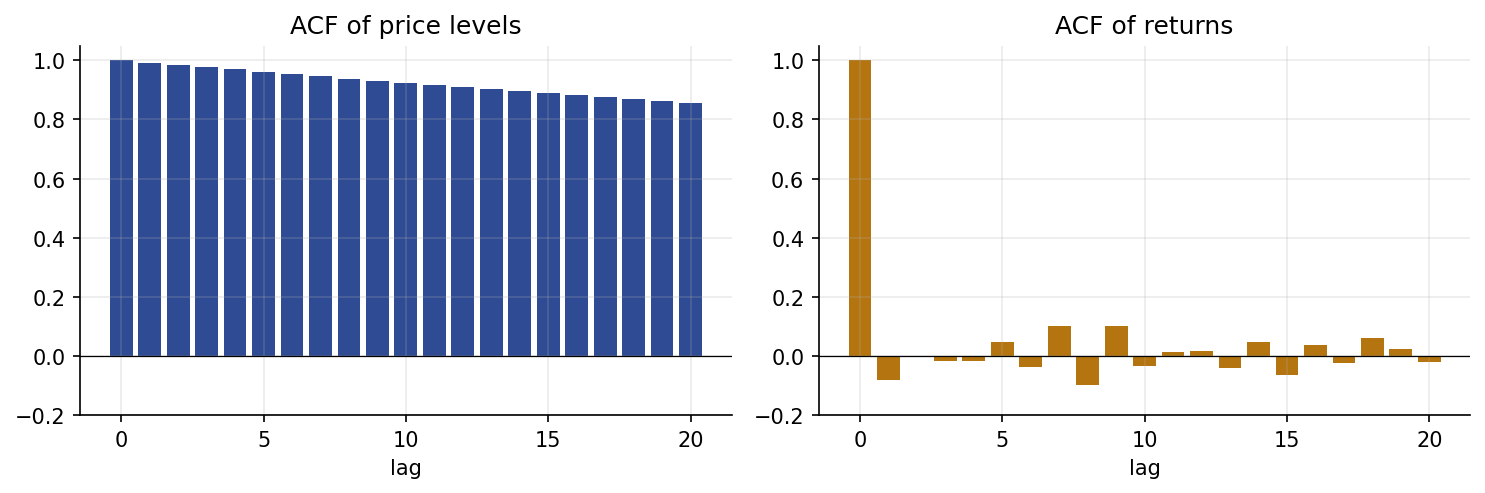
\includegraphics[width=\columnwidth]{fig_eda_acf.png}
\caption{Autocorrelation: price levels (left) are near-unit-root; returns (right)
are effectively white. Predicting levels exploits the left panel.}
\label{fig:eda_acf}
\end{figure}

\begin{figure}[t]
\centering
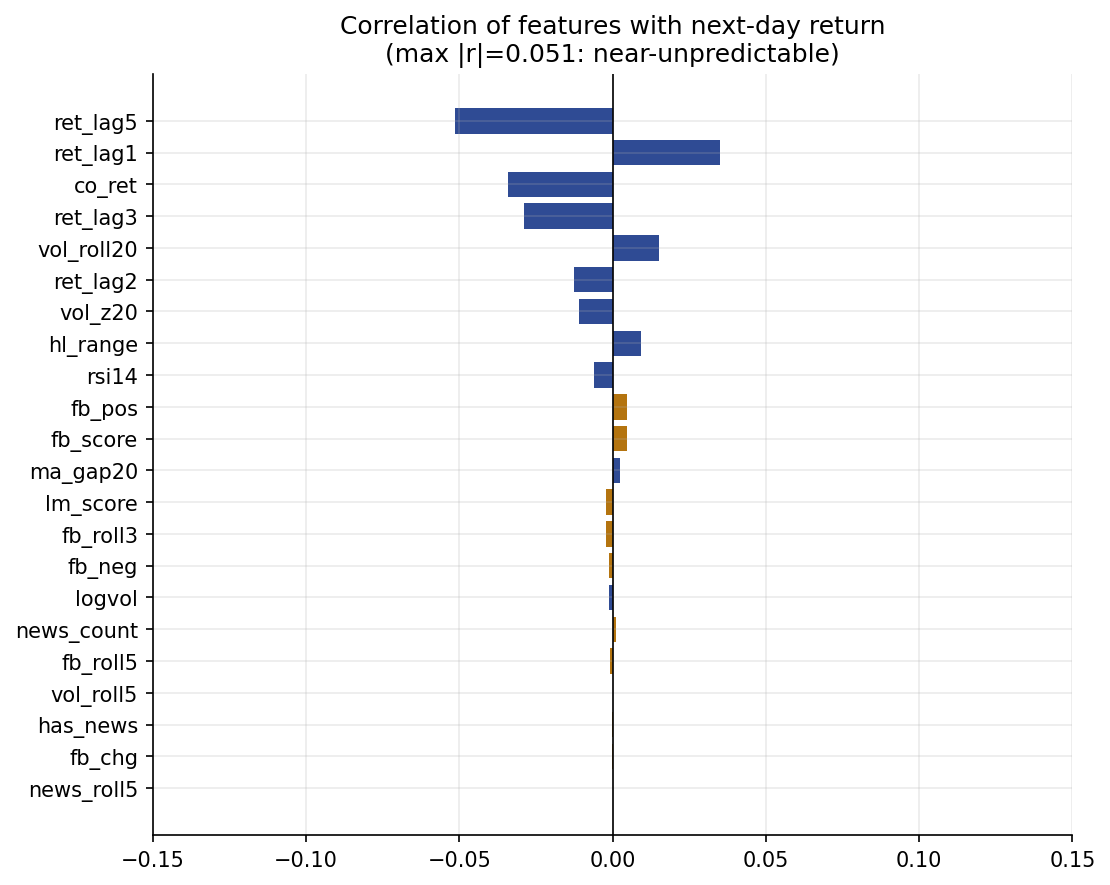
\includegraphics[width=0.82\columnwidth]{fig_eda_feat_target.png}
\caption{Correlation of each backward-looking feature with the next-day return.
The maximum is $\edaFeatTargetMax$; sentiment features (orange) are near zero.}
\label{fig:eda_feat}
\end{figure}

\begin{figure}[t]
\centering
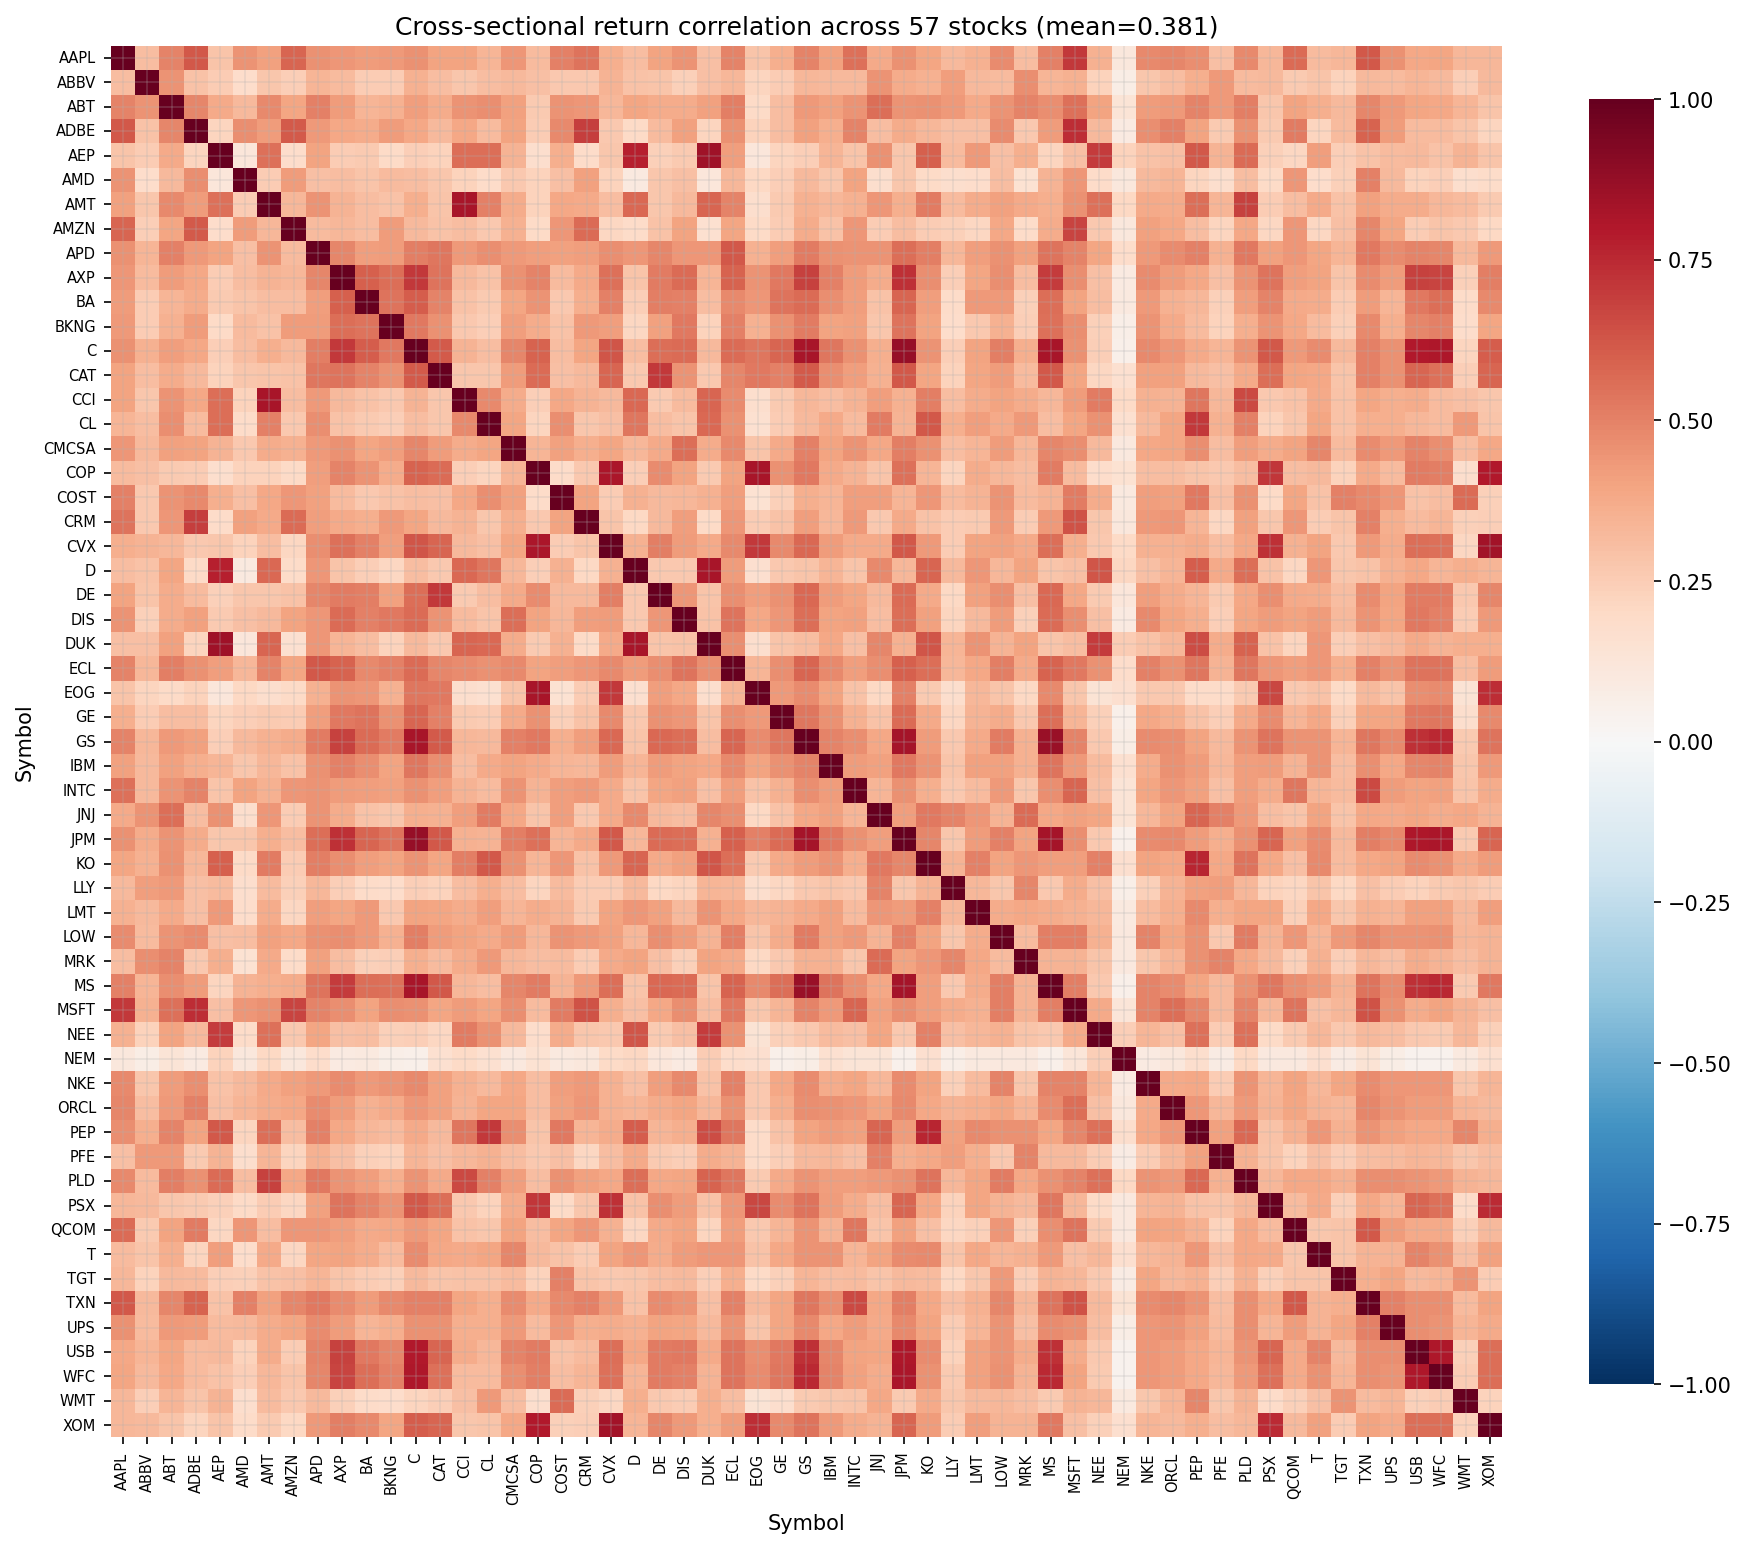
\includegraphics[width=0.82\columnwidth]{fig_eda_cross_corr.png}
\caption{Cross-sectional return correlation across all 57 stocks in the
universe (mean $\edaCrossCorr$): observations are not independent, motivating
symbol-clustered inference.}
\label{fig:eda_cross}
\end{figure}

\begin{figure}[t]
\centering
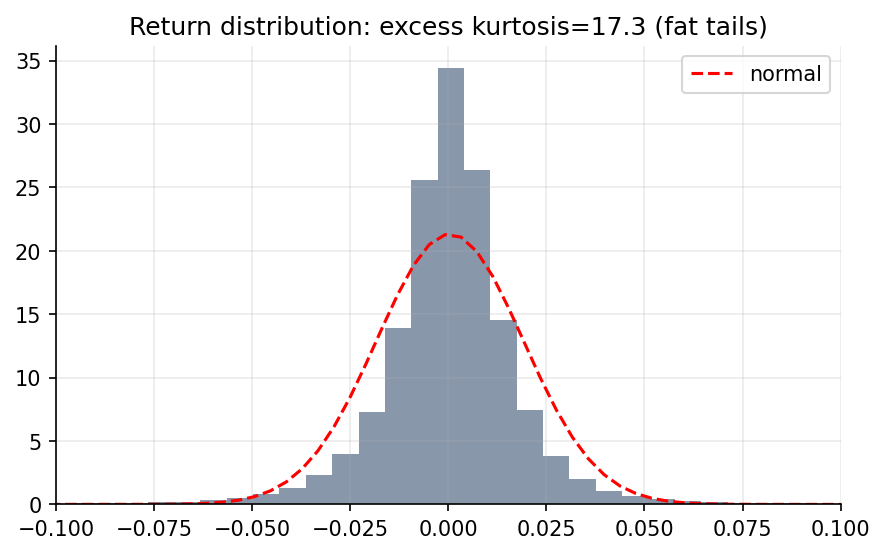
\includegraphics[width=0.9\columnwidth]{fig_eda_return_dist.png}
\caption{Return distribution after data cleaning: fat-tailed
(excess kurtosis $\edaKurtosis$) but free of the splice artifacts that
originally produced kurtosis $>\!4000$.}
\label{fig:eda_dist}
\end{figure}

\section{The Illusion of Skill: A Leakage Study}
\label{sec:leakage}
We first reproduce the standard ``high-accuracy'' setup and dissect it.
Table~\ref{tab:leakage} and Fig.~\ref{fig:leakage} report four experiments with
the \emph{same} Random Forest.

\begin{table}[t]
\caption{Next-day prediction under different protocols (Random Forest).
Random-split level prediction reproduces $R^2\approx0.99$, but a persistence
baseline matches it and the honest return task collapses.}
\label{tab:leakage}
\centering
\begin{tabular}{@{}llrr@{}}
\toprule
Protocol & Target & $R^2$ & RMSE \\
\midrule
RF, random split & level & 0.999 & 6.992 \\
RF, chronological & level & 0.994 & 26.028 \\
Persistence $\hat P_{t+1}{=}P_t$ & level & 1.000 & 7.158 \\
RF, chronological & \textbf{return} & -0.033 & 0.019 \\
\bottomrule
\end{tabular}

\end{table}

\begin{figure}[t]
\centering
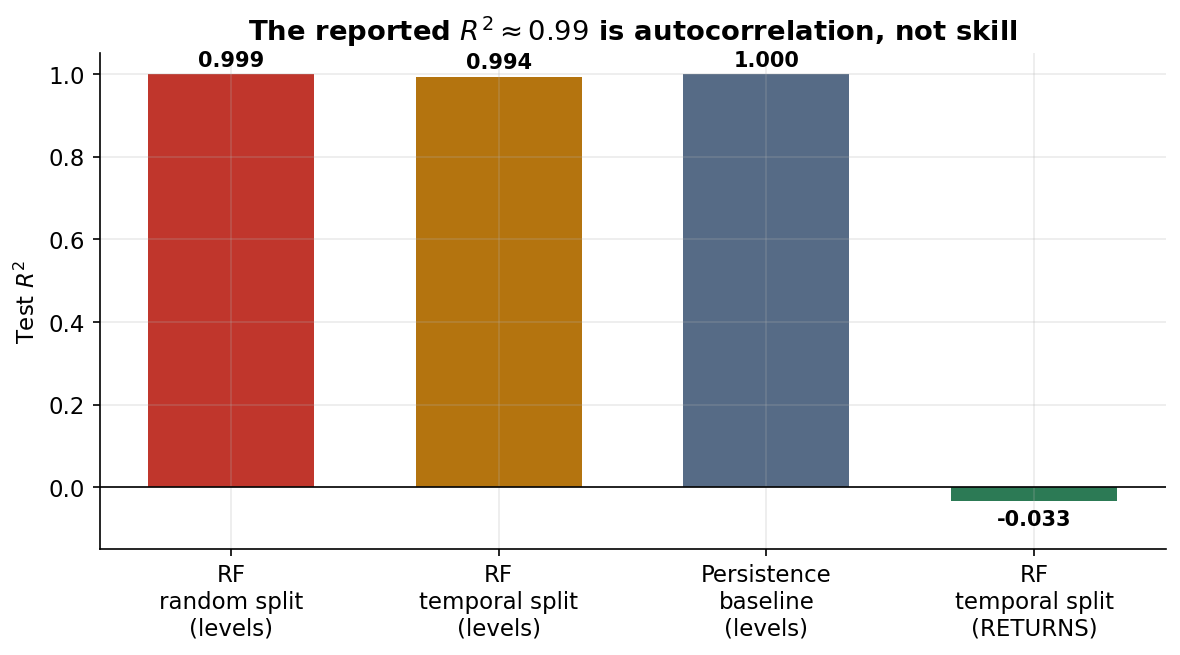
\includegraphics[width=\columnwidth]{fig_leakage.png}
\caption{The reported $R^2\approx0.99$ is autocorrelation, not skill. A naive
persistence baseline equals the model on levels; predicting returns yields
$R^2<0$.}
\label{fig:leakage}
\end{figure}

The random-split level model attains $R^2=\RleakRand$; keeping the same
features and target but using a chronological split barely changes it
($R^2=\RleakChrono$), because the ``skill'' is autocorrelation, not the split.
The decisive comparison is the persistence baseline $\hat P_{t+1}=P_t$, which
attains $R^2=\RleakPersist$---indistinguishable from the model. When the same
model instead predicts \emph{returns}, performance falls to
$R^2=\RleakReturns$, i.e.\ worse than predicting a constant zero. Level-scale
$R^2$ is therefore not a meaningful measure of forecasting skill here.

\section{Correlation Structure of the Data}
\label{sec:collinearity}
A second hazard---and the one most likely to threaten conclusions in this
literature---is the strong correlation \emph{among} features, \emph{across}
stocks, and \emph{across} time. We treat it as a first-class threat to validity.

\textbf{Three kinds of correlation.} (i) \emph{Feature multicollinearity}:
Fig.~\ref{fig:vif} reports variance inflation factors (VIF); the raw OHLCV levels
used by prior pipelines are near-perfectly collinear (VIF up to $\vifClose$,
versus the usual threshold of 10), which destabilizes linear coefficients and
invalidates PDP- and coefficient-based explanations. (ii) \emph{Temporal
autocorrelation}: price levels are near-unit-root and overlapping features are
serially correlated, so IID cross-validation and IID significance tests are
invalid. (iii) \emph{Cross-sectional correlation}: the stocks co-move with the
market, so pooled stock-day observations are far from independent and naive tests
overstate significance.

\textbf{Why our conclusion is robust to all three.} Crucially, our central claim
is a \emph{null} (news sentiment adds no measurable value). Correlation threatens
a null in only one way---by \emph{masking} a real effect behind correlated price
features---and we rule this out directly: the \emph{sentiment-only} models
(Sec.~\ref{sec:results}) test sentiment in complete isolation and still achieve no
skill ($R^2\!\le\!0$, MCC$\approx\!0$), so no price feature can be hiding it. The
other failure mode of correlation---\emph{inflating} apparent significance---can
only make a positive claim look stronger, and we make no positive claim; we
nonetheless guard against it so our ``no-effect'' confidence intervals are honest.
Concretely we use: stationary transforms (returns, ratios, $z$-scores; max VIF
$\vifStatMax$, a $\sim$17$\times$ reduction); ALE~\cite{apley2020ale} and
\emph{grouped} attribution rather than PDP or per-feature bars; \emph{grouped
block-permutation} importance that permutes the entire sentiment block jointly
(preserving within-block correlation, so redundancy cannot hide the block's
contribution); embargoed walk-forward splits; a \emph{symbol-clustered} bootstrap
that resamples whole stocks (respecting cross-sectional dependence); and
Newey--West HAC Diebold--Mariano tests (respecting temporal dependence). Every
significance statement below uses stocks, not stock-days, as the effective unit.

\begin{figure}[t]
\centering
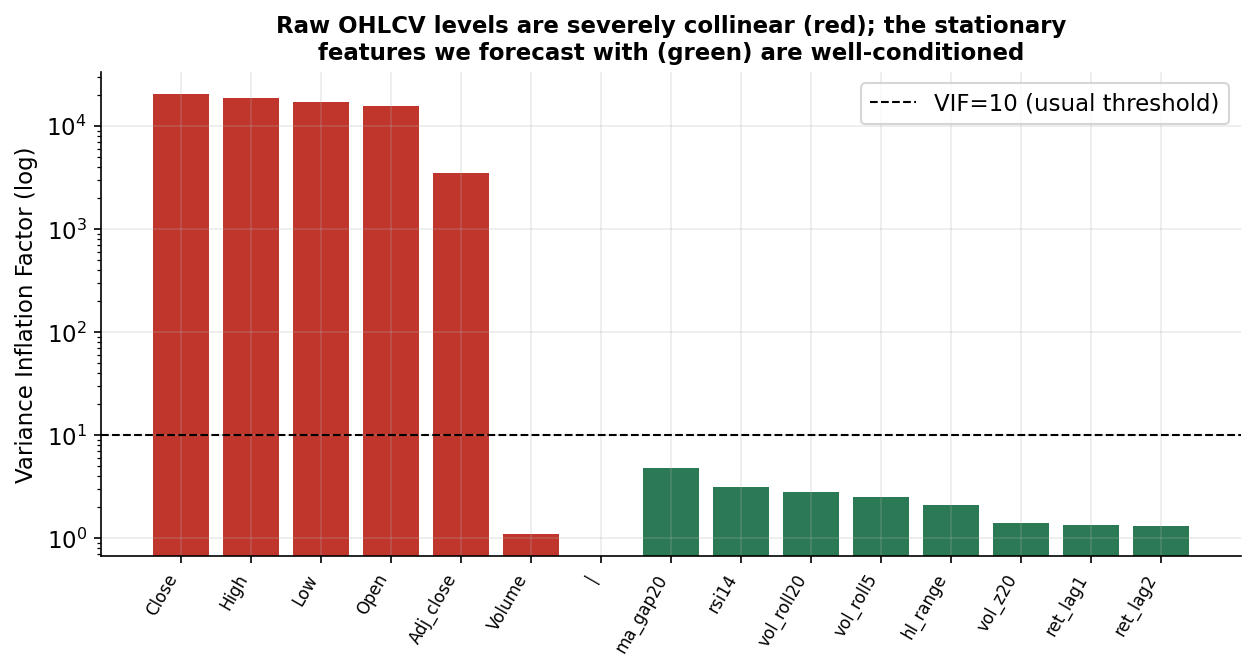
\includegraphics[width=\columnwidth]{fig_vif.png}
\caption{Variance inflation factors. Raw OHLCV levels (red) are severely
collinear; the stationary features we use (green) are well conditioned.}
\label{fig:vif}
\end{figure}

\section{Leakage-Free Evaluation}
\textbf{Protocol.} We use an expanding-window walk-forward: for each test year
$Y\in\{2021,2022,2023\}$ we train on all data before $Y$ (with a 10-day
embargo) and test on $Y$. Features are standardized on the training fold only.
We report per-fold metrics and their mean.

\textbf{Models and baselines.} Ridge/Logistic, Random Forest, XGBoost,
LightGBM, SVM, and a two-layer GRU. Baselines: persistence and historical-mean
returns (regression) and majority-class/always-up (direction).

\textbf{Ablation.} Each model is trained on \emph{price-only},
\emph{sentiment-only}, and \emph{price$+$sentiment} feature sets, isolating the
marginal contribution of news.

\begin{table*}[t]
\caption{Leakage-free walk-forward results (mean over test years 2021--2023).
No model beats the naive baselines on returns; directional accuracy is near
chance; adding sentiment does not help.}
\label{tab:main}
\centering
\footnotesize
\setlength{\tabcolsep}{4pt}
\begin{tabular}{@{}l|rrr|rrr@{}}
\toprule
& \multicolumn{3}{c|}{Return ($R^2$ / RMSE / DirAcc)} & \multicolumn{3}{c}{Direction (Acc / F1 / MCC)} \\
Model & \multicolumn{3}{c|}{} & \multicolumn{3}{c}{} \\
\midrule
\multicolumn{7}{@{}l}{\emph{Baselines}}\\
~~persistence/zero & -0.001 & 0.021 & -- & -- & -- & -- \\
~~hist.\ mean / majority & -0.001 & 0.021 & -- & 0.513 & 0.678 & 0.000 \\
\midrule
Ridge (price) & -0.009 & 0.022 & 0.504 & 0.513 & 0.638 & 0.014 \\
Ridge (+sent) & -0.010 & 0.022 & 0.504 & 0.512 & 0.638 & 0.011 \\
\addlinespace
RandomForest (price) & -0.013 & 0.022 & 0.512 & 0.503 & 0.530 & 0.004 \\
RandomForest (+sent) & -0.012 & 0.022 & 0.512 & 0.501 & 0.527 & 0.001 \\
\addlinespace
XGBoost (price) & -0.015 & 0.022 & 0.509 & 0.510 & 0.622 & 0.006 \\
XGBoost (+sent) & -0.014 & 0.022 & 0.509 & 0.509 & 0.621 & 0.004 \\
\addlinespace
LightGBM (price) & -0.018 & 0.022 & 0.505 & 0.509 & 0.615 & 0.004 \\
LightGBM (+sent) & -0.016 & 0.022 & 0.508 & 0.508 & 0.613 & 0.003 \\
\addlinespace
SVR (price) & -0.511 & 0.025 & 0.489 & 0.510 & 0.606 & 0.011 \\
SVR (+sent) & -0.542 & 0.026 & 0.490 & 0.508 & 0.597 & 0.009 \\
\addlinespace
\bottomrule
\end{tabular}

\end{table*}

\subsection{Results}
\label{sec:results}
Table~\ref{tab:main} summarizes the honest tasks. On next-day \textbf{returns},
every model's $R^2$ is near zero or negative---none beats the persistence or
historical-mean baseline (Fig.~\ref{fig:returns}). On \textbf{direction}, the
best model reaches $\bestDirAcc\%$ accuracy versus a $\majAcc\%$ majority
baseline, with Matthews correlation near zero (Fig.~\ref{fig:mcc}). Performance
is weak but stable across regimes, including the 2022 drawdown
(Fig.~\ref{fig:wf}). Importantly, the \emph{sentiment-only} models---which
isolate news from all price information---are no better than chance, establishing
that sentiment carries no standalone next-day signal here and that its
non-contribution in the combined model is not an artifact of price features
masking it.

\begin{figure}[t]
\centering
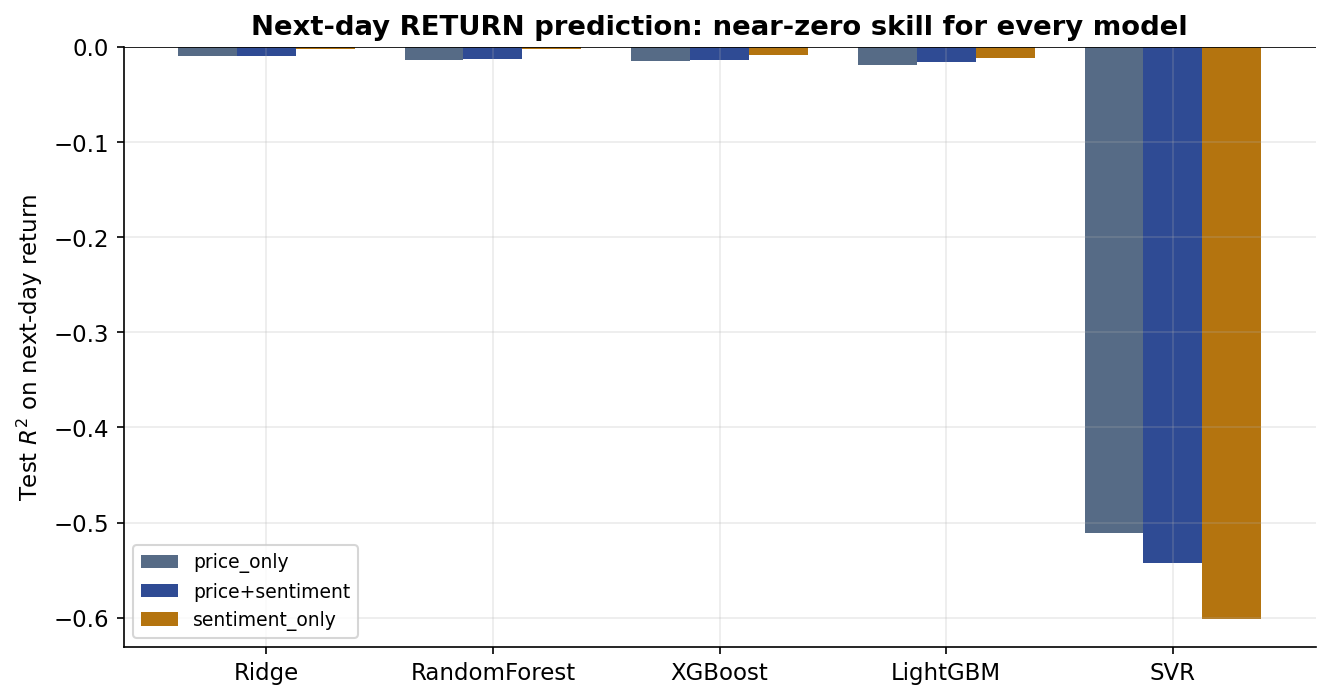
\includegraphics[width=\columnwidth]{fig_returns_r2.png}
\caption{Next-day return $R^2$ by model and feature set. All near zero;
sentiment does not shift the picture.}
\label{fig:returns}
\end{figure}

\begin{figure}[t]
\centering
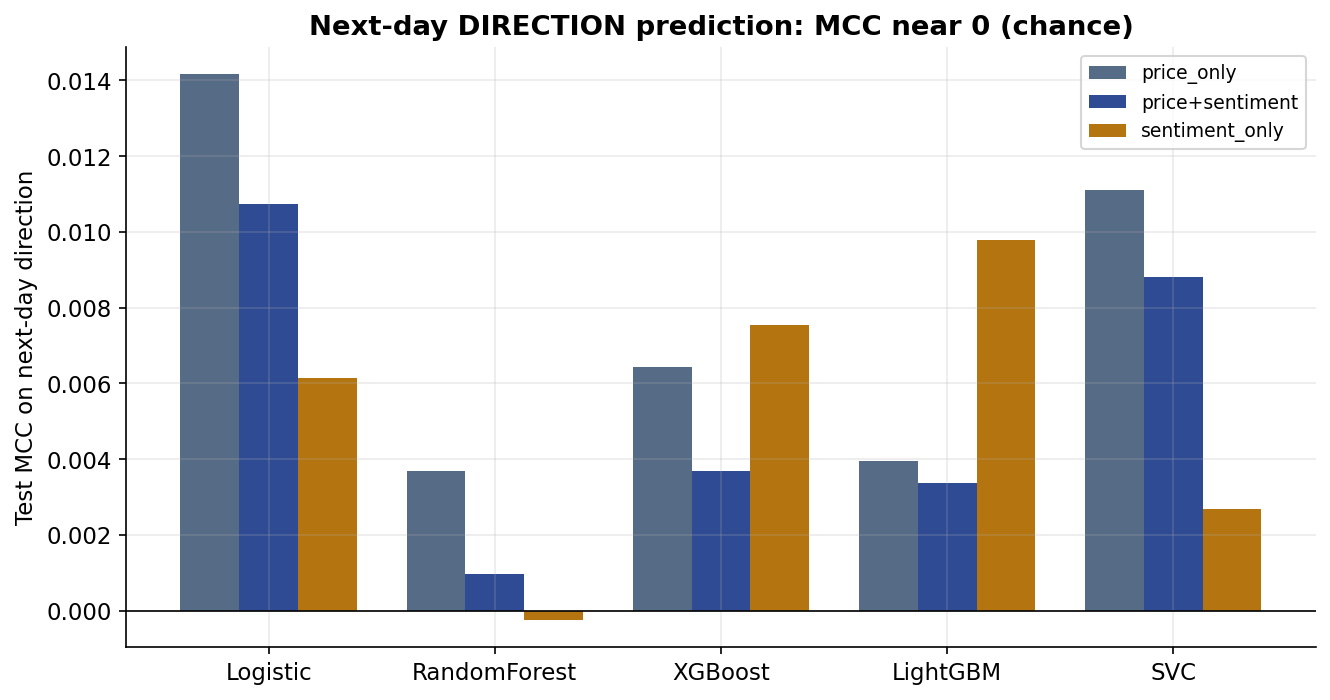
\includegraphics[width=\columnwidth]{fig_direction_mcc.png}
\caption{Directional MCC by model and feature set. Near-zero (chance) for all.}
\label{fig:mcc}
\end{figure}

\begin{figure}[t]
\centering
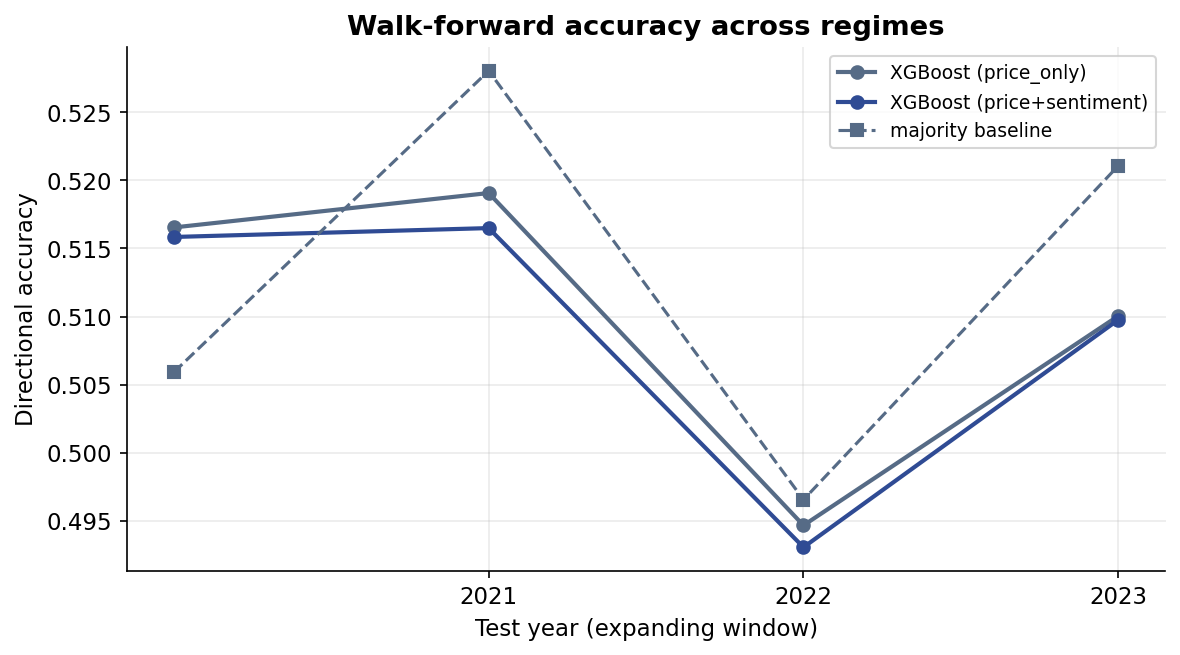
\includegraphics[width=\columnwidth]{fig_walkforward.png}
\caption{Walk-forward directional accuracy across regimes (2021--2023).}
\label{fig:wf}
\end{figure}

\subsection{Does news sentiment help? A dependence-aware test}
Table~\ref{tab:ablation} reports the marginal value of sentiment. Adding news
features changes directional accuracy by $\sentDeltaAcc$ percentage points, with
a 95\% symbol-clustered bootstrap CI of $[\sentCIlo,\sentCIhi]$ that straddles
zero; Wilcoxon tests across symbols are non-significant. For returns, HAC
Diebold--Mariano tests find no consistent reduction in forecast error
(Fig.~\ref{fig:ablation}). We report XGBoost's result as representative of the
tree-ensemble/kernel majority of the zoo, but it is not universal: Logistic
Regression's clustered CI on the same ablation, $[-0.26,-0.02]$ percentage
points (Table~\ref{tab:ablation}), excludes zero (Wilcoxon $p=0.06$, borderline),
a small but directionally consistent \emph{negative} effect of adding
sentiment features for that one linear model. We do not present XGBoost's
null as representative of every model in the zoo; the honest summary is
model-dependent near-zero effects, mostly indistinguishable from noise, with
one linear-model exception that itself argues against sentiment adding value
rather than for it.

\begin{table}[t]
\caption{Marginal value of news sentiment (price$+$sentiment vs.\ price-only),
with dependence-aware inference.}
\label{tab:ablation}
\centering\scriptsize
\begin{tabular}{@{}lrrrr@{}}
\toprule
Model & $\Delta$Acc (pp) & 95\% CI & Wilcoxon $p$ & DM $t$ (HAC) \\
\midrule
Logistic & -0.14 & $[-0.26,-0.02]$ & 0.06 & -- \\
XGBoost & -0.13 & $[-0.39,0.14]$ & 0.51 & 0.17 \\
LightGBM & -0.04 & $[-0.36,0.26]$ & 0.97 & 0.09 \\
\bottomrule
\end{tabular}

\end{table}

\begin{figure}[t]
\centering
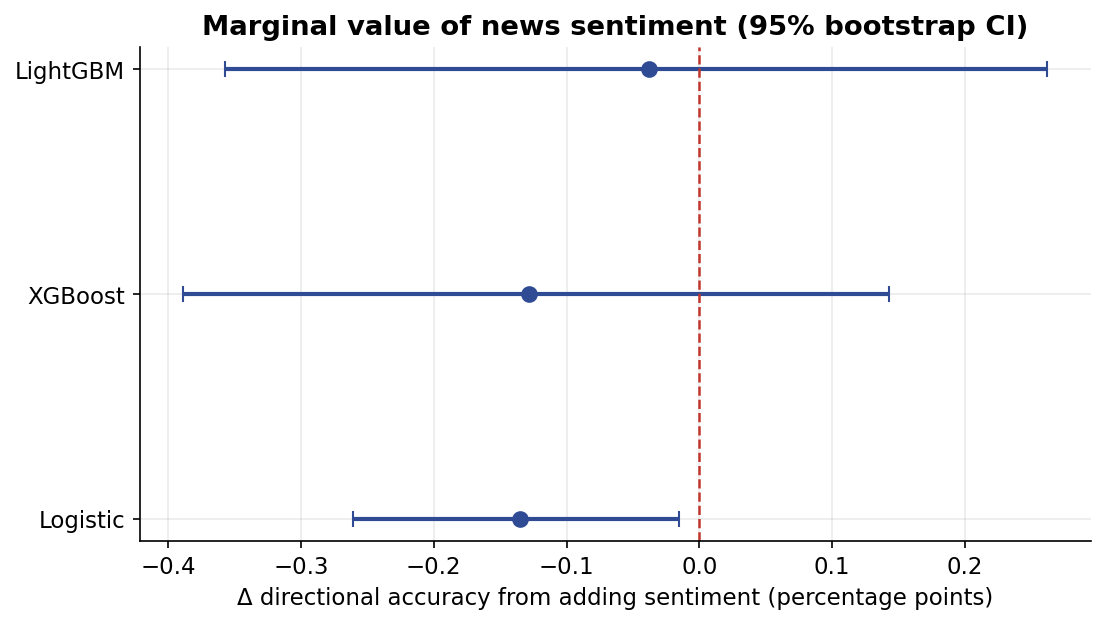
\includegraphics[width=\columnwidth]{fig_ablation.png}
\caption{Change in directional accuracy from adding sentiment, with 95\%
symbol-clustered bootstrap CIs. All intervals include zero.}
\label{fig:ablation}
\end{figure}

\section{Explainability: Attribution Is Not Predictive Value}
\label{sec:xai}
Applying explainability here yields a cautionary lesson rather than a simple
verdict, and interpreting it carefully matters. \emph{In-sample} attribution
assigns news sentiment a sizable role: SHAP gives the ten sentiment features
$\shapSentShare\%$ of total importance (Fig.~\ref{fig:shap}) and the GRU's
Integrated Gradients give sentiment channels $\igSentShare\%$
(Fig.~\ref{fig:xai2}). Read naively, this looks like evidence that sentiment
matters.

It is not. Attribution measures how a flexible model \emph{uses} features to fit
the training data, not their out-of-sample predictive value---and the two diverge
sharply here. The correlation-robust \emph{grouped block-permutation} test, which
permutes the entire sentiment block jointly so within-group redundancy cannot hide
a real effect, changes test accuracy by only $\blockPermSent$ points---within
noise, and no larger than for the price block ($\blockPermPrice$ points) on this
near-unpredictable task (Fig.~\ref{fig:blockperm}). ALE curves for sentiment
features are nearly flat, and the sentiment-only models (Sec.~\ref{sec:results})
have no skill. Thus the large SHAP/IG share reflects in-sample fitting of noise,
not signal. The methodological takeaway, relevant to the wider use of XAI in
finance, is that a large attribution share is not evidence of predictive value;
the ablation and block-permutation tests, not the attribution bars, settle the
question.

\begin{figure}[t]
\centering
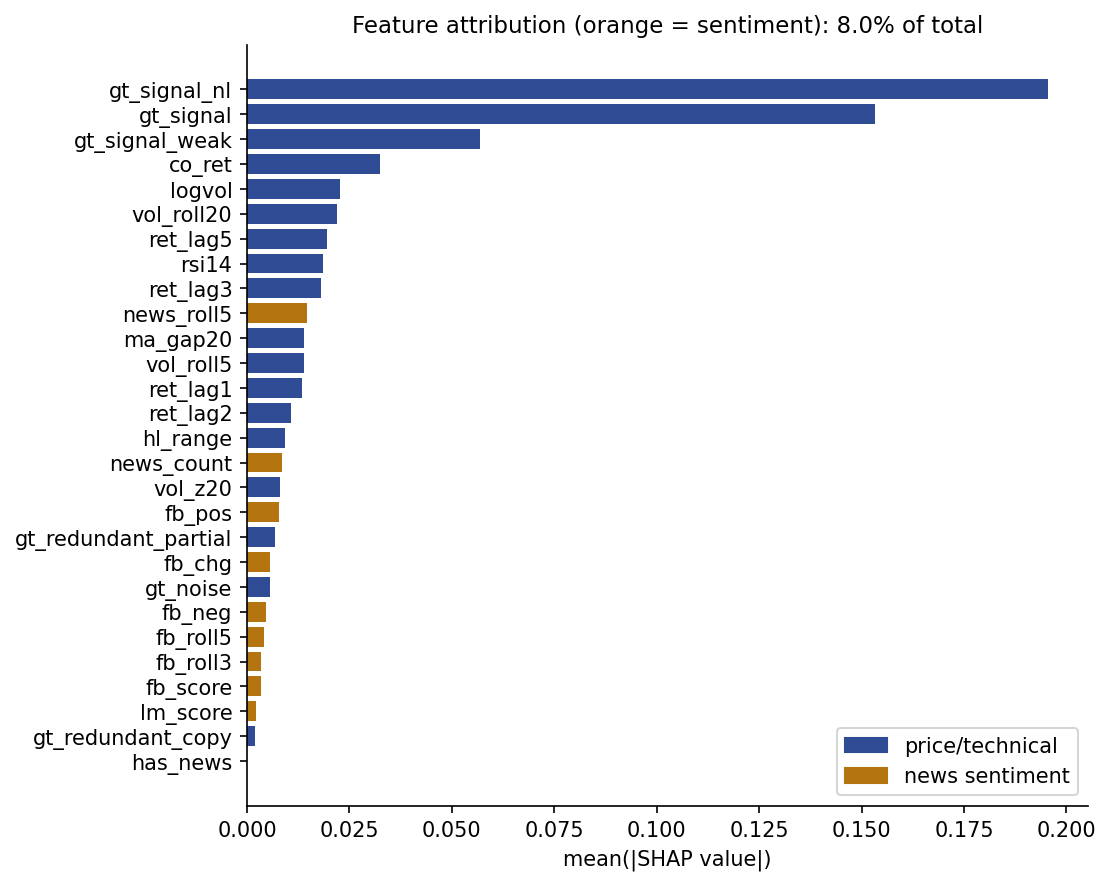
\includegraphics[width=\columnwidth]{fig_shap_grouped.png}
\caption{Grouped SHAP attribution (orange: news sentiment). Sentiment receives a
sizable \emph{in-sample} share ($\shapSentShare\%$)---which, as
Fig.~\ref{fig:blockperm} shows, does not translate to out-of-sample value.}
\label{fig:shap}
\end{figure}

\begin{figure}[t]
\centering
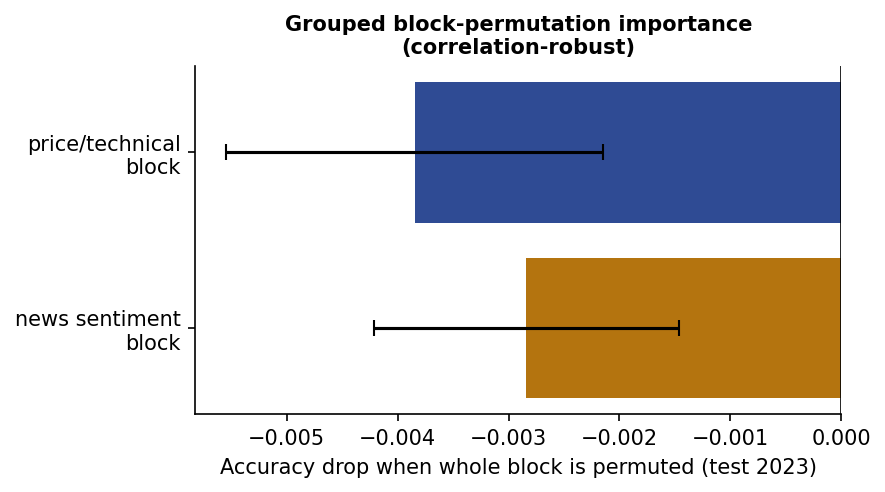
\includegraphics[width=0.82\columnwidth]{fig_block_perm.png}
\caption{Correlation-robust grouped block-permutation. Jointly permuting the news
sentiment block changes accuracy by only $\blockPermSent$ pp (within noise),
despite sentiment's large SHAP share; next-day direction is near-unpredictable
from either feature group.}
\label{fig:blockperm}
\end{figure}

\begin{figure}[t]
\centering
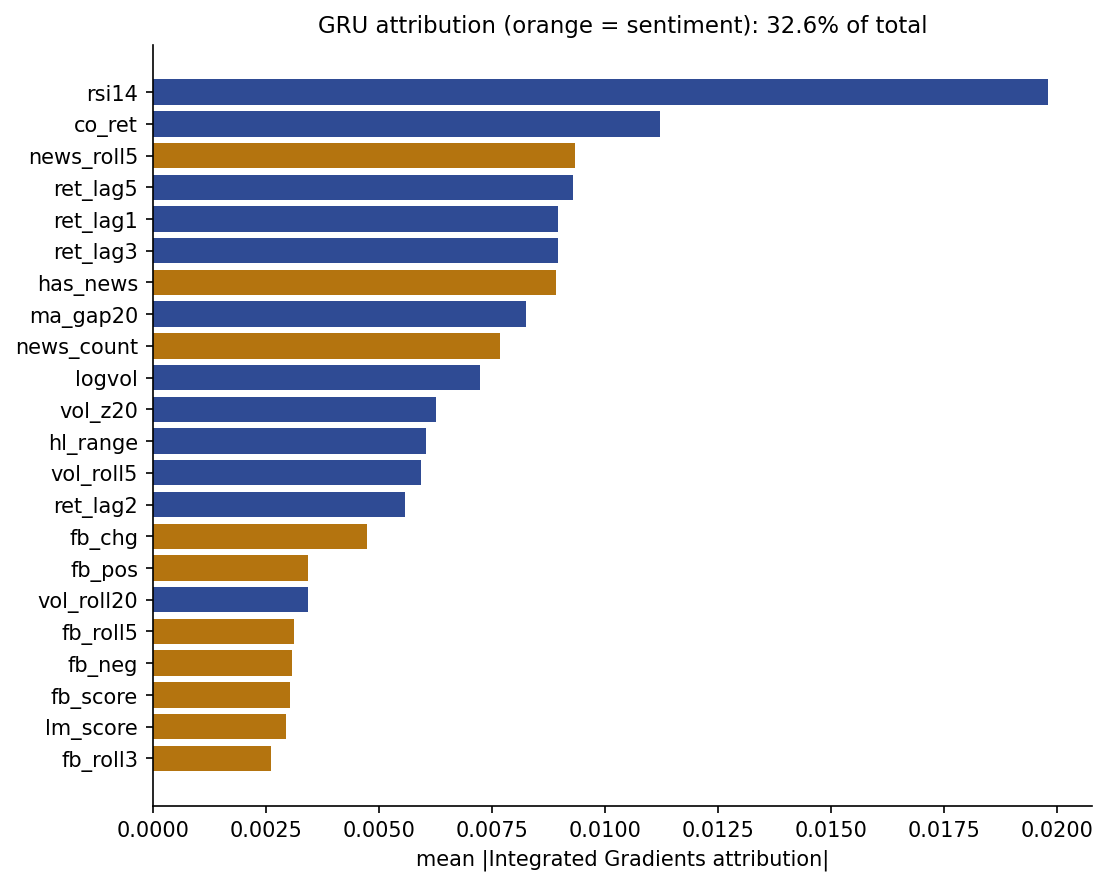
\includegraphics[width=0.86\columnwidth]{fig_ig_gru.png}
\caption{GRU Integrated-Gradients attribution. Sentiment channels (orange) get a
large in-sample share, again not reflected in out-of-sample performance.}
\label{fig:xai2}
\end{figure}

\section{Model Zoo}
\label{sec:zoo}
To make faithfulness a function of model class (RQ3) rather than a single
case study, we train \nModelsZoo{} models spanning seven families on the
identical panel and walk-forward protocol: linear/glass-box (Ridge/Logistic),
a single decision tree, tree ensembles (Random Forest, XGBoost, LightGBM,
CatBoost), kernel/instance-based (SVM, $k$-NN), a GAM (EBM), dense/recurrent/
convolutional/attention neural networks (MLP, GRU, LSTM, 1D-CNN, TCN, a small
Transformer), and a graph neural network over a static cross-stock
correlation graph (top-5 $|\rho|$ neighbors, built from training-fold returns
only, to avoid leaking future co-movement structure into the graph). All are
evaluated on the same direction/return tasks; Table~\ref{tab:zoo} reports
directional accuracy, F1, and MCC for the price+sentiment feature set,
averaged over the \faithUniverseN{}-stock, four-fold walk-forward.

\begin{table}[t]
\centering\tiny
\caption{Model zoo, direction task (price+sentiment, mean over folds). Near-chance
accuracy and near-zero MCC across every family is the expected result on this
validated near-zero-signal test-bed, not a modelling failure. $\pm$ values
are the half-width of a stock-clustered 95\% CI (5000 resamples, whole
symbols, matching Table~\ref{tab:faithfulness}'s protocol) where per-symbol
predictions were cached (XGBoost, LightGBM, Logistic, $\nModelsZooCiScored{}$
models); see text.}
\begin{tabular}{@{}llrrr@{}}
\toprule
Model & Family & Acc & F1 & MCC \\
\midrule
Transformer & attention & 0.504 & 0.590 & -0.003 \\
CatBoost & classical/ML & 0.510 & 0.637 & 0.003 \\
DecisionTree & classical/ML & 0.501 & 0.493 & 0.003 \\
EBM & classical/ML & 0.506 & 0.583 & 0.005 \\
KNN & classical/ML & 0.502 & 0.554 & 0.001 \\
LightGBM & classical/ML & 0.508$\pm$0.004 & 0.613$\pm$0.013 & 0.003$\pm$0.007 \\
Logistic & classical/ML & 0.512$\pm$0.004 & 0.638$\pm$0.015 & 0.011$\pm$0.008 \\
MLP & classical/ML & 0.508 & 0.608 & 0.005 \\
RandomForest & classical/ML & 0.501 & 0.527 & 0.001 \\
SVC & classical/ML & 0.508 & 0.597 & 0.009 \\
XGBoost & classical/ML & 0.509$\pm$0.005 & 0.621$\pm$0.013 & 0.004$\pm$0.008 \\
CNN1d & conv & 0.507 & 0.590 & 0.002 \\
TCN & conv & 0.508 & 0.546 & 0.004 \\
GNN & graph & 0.502 & 0.598 & -0.006 \\
GRU & recurrent & 0.500 & 0.547 & -0.003 \\
LSTM & recurrent & 0.505 & 0.572 & 0.002 \\
\bottomrule
\end{tabular}

\label{tab:zoo}
\end{table}

Mean accuracy across the zoo is $\modelZooMeanAcc$ (majority-class baseline:
$\majAcc\%$) and the largest-magnitude MCC across all \nModelsZoo{} models is
only $\modelZooMaxMCC$. This is the validated substrate the faithfulness
benchmark stress-tests: no model family finds exploitable real-world signal,
so any method that reports large, confident importance for a \emph{real}
(non-ground-truth) feature on this substrate is reporting something the data
does not support.

\textbf{Interval-aware reporting (M6, addressing a specific reviewer
question).} Table~\ref{tab:zoo} reports point Acc/F1/MCC for all
\nModelsZoo{} models; $\nModelsZooCiScored{}$ of them (XGBoost, LightGBM,
Logistic) additionally carry a real stock-clustered 95\% CI, computed from
cached per-symbol predictions with the identical whole-symbol-resampling
protocol as the faithfulness benchmark (Section~\ref{sec:faithfulness}). For
the remaining models we do not fabricate an interval: per-symbol predictions
are not yet cached for them, so no bootstrap is possible without a further
training pass. The caution this omission calls for is the same one already
argued from Section~\ref{sec:collinearity}'s $\bar\rho=\edaCrossCorr$
cross-sectional dependence and $\faithEffN$ effective sample size---every
point estimate in Table~\ref{tab:zoo} should be read as resting on
$\faithEffN$, not $\faithUniverseN$, independent units, whether or not its
row carries an explicit bracket. Extending real per-symbol CIs to the full
zoo is a direct, mechanical extension of the existing pipeline and is left
as immediate future work rather than papered over.

\section{The XAI Method Suite and Applicability}
\label{sec:xaisuite}
We organize methods by taxonomy---attribution, rule/example-based,
concept-based, gradient/propagation, graph, and mechanistic---and apply each
only to model classes it is architecturally valid for (never force-fit; an
inapplicable cell is reported as such, which we treat as a credibility gain,
not a gap). Every neural, convolutional, attention, and graph model is given a
ground-truth-augmented version of its inputs specifically for this scoring
(Section~\ref{sec:groundtruth}), so a method being N/A here reflects a genuine
architectural limit (e.g.\ captum's LRP has no propagation rule for a
recurrent layer), not a missing artifact. Table~\ref{tab:catalogue} is the
applicability matrix and per-method faithfulness summary, reported separately
for the linear (\texttt{gt\_signal}) and nonlinear (\texttt{gt\_signal\_nl})
planted signals. ``Faithful?'' reports, for methods that yield a global
importance vector, whether the corresponding planted signal ranks above
\texttt{gt\_noise} (aggregated as $k/n$ across the $n$ applicable models where
more than one was tested); for methods evaluated on other criteria per
convention (rule/example methods on precision/coverage or validity/sparsity;
mechanistic methods on their own honest verdict), that criterion is reported
instead and the nonlinear column is left blank (not applicable to a
precision/coverage or validity/sparsity criterion).

\textbf{What the Note column means (M3).} Every row in Table~\ref{tab:catalogue},
including TreeSHAP/KernelSHAP/LIME/permutation, reports a single-fit credit
share averaged across that method's applicable \emph{models} (tagged
\emph{avg./$k$ models} when $k{>}1$)---\emph{not} the stock-clustered value.
This column and Table~\ref{tab:faithfulness}'s Credit column average over two
different axes (models here, stocks there) and are not interchangeable; we
label both explicitly rather than let the same-looking numbers be conflated.
The genuinely stock-clustered credit share exists only for the four core
methods, in Table~\ref{tab:faithfulness}. For methods evaluated on other
criteria (precision, coverage, validity, sparsity, TCAV score, etc.), that
metric is self-labeled instead. Extending stock-clustered per-symbol
treatment to every neural/graph method is a natural next step
(Section~\ref{sec:limits}), not yet part of this release.

\begin{table*}[t]
\centering\tiny
\caption{XAI method catalogue: family, applicable model(s), and faithfulness
verdict against both the linear and nonlinear planted signal. The Grad-CAM
family's native output is a per-timestep curve, not a per-feature vector, so
its faithfulness score is reported via a paired per-feature Integrated-
Gradients pass on the same ground-truth-augmented CNN1d model (documented in
the note column); Grad-CAM/++/Score-CAM remain restricted to the 1D-CNN as a
vision-native family, never applied to non-convolutional models.}
\begin{tabular}{@{}llllll@{}}
\toprule
Method & Family & Applicable model(s) & Faithful (linear) & Faithful (nonlinear) & Note \\
\midrule
treeshap & attribution & 5 tree models & 5/5 yes & 5/5 yes & 0.34 (avg./4 models) \\
kernelshap & attribution & Logistic/RF/XGBoost/EBM/SVM & 5/5 yes & 5/5 yes & 0.44 (avg./5 models) \\
lime & attribution & Logistic/RF/XGBoost/EBM/SVM & 5/5 yes & 5/5 yes & 0.48 (avg./5 models) \\
permutation & attribution & Logistic/RF/XGBoost/EBM/SVM & 5/5 yes & 5/5 yes & 0.53 (avg./3 models) \\
integrated\_gradients & gradient & GRU/LSTM/CNN1d/TCN/Transformer & 5/5 yes & 5/5 yes & 0.52 (avg./5 models) \\
rise & attribution (adapted) & XGBoost & yes & yes & 0.37 \\
ebm\_intrinsic & intrinsic & EBM & yes & yes & 0.47 \\
gam\_aggregation & global aggregation & XGBoost (TreeSHAP-derived) & yes & yes & 0.42 \\
muse\_brcg & rule surrogate & XGBoost & yes & yes & -- \\
lrp & gradient/propagation & MLP (GRU: N/A, no supported layers) & yes & yes & 0.44 \\
guided\_backprop & gradient/propagation & MLP & yes & yes & 0.49 \\
deconvnet & gradient/propagation & MLP & yes & yes & 0.90 \\
gnnexplainer & graph & GNN & yes & yes & 0.49 \\
anchors & rule/example & XGBoost & precision=0.92 & -- & coverage=0.035 \\
counterfactual & rule/example & XGBoost & validity=1.00 & -- & sparsity=1.27 \\
cem & rule/example & XGBoost & PP size=0.13 & -- & -- \\
tcav (high\_attention) & concept & GRU & TCAV=1.00 & -- & CAV acc=0.88 \\
tcav (positive\_sentiment) & concept & GRU & TCAV=1.00 & -- & CAV acc=0.78 \\
gradcam & CAM (vision-native) & CNN1d only & yes & -- & 0.55 \\
gradcam\_pp & CAM (vision-native) & CNN1d only & yes & -- & 0.55 \\
score\_cam & CAM (vision-native) & CNN1d only & yes & -- & 0.55 \\
sae & mechanistic & Transformer & 253/256 interp. & -- & thr.\ $|r|{>}$0.3 \\
acdc (ablation) & mechanistic & Transformer & 0 notable/10 & -- & z{>}2.0 \\
\bottomrule
\end{tabular}

\label{tab:catalogue}
\end{table*}

\textbf{What ``muse\_brcg'' is.} It combines two global-surrogate
techniques, not one algorithm: MUSE selects an interpretable input subspace;
BRCG (Boolean Rule Column Generation) fits a compact Boolean rule list on it
to approximate the black box. Our 8-leaf surrogate of the XGBoost classifier
has high fidelity to the black box's own predictions but only near-chance
accuracy against true labels---the expected, consistent combination for a
faithful surrogate of an unskilled model, not a contradiction.

Of the $\nXaiMethodsCatalogued$ methods catalogued, $\nXaiFaithfulOfScoreable$
are scoreable against ground truth and every one of them correctly ranks the
planted signal above pure noise --- for both the linear and the nonlinear
signal, wherever both were checked. This is a substantially larger scoreable
set than a single-model, tabular-only check would give: Integrated Gradients
now has a real score on all five sequence architectures, and the Grad-CAM
family, while still restricted to the CNN1d for its native temporal output, no
longer reports a blanket N/A for feature-level faithfulness. The remaining
non-scoreable rows are genuine architectural limits (captum's LRP has no rule
for a recurrent layer; CAM's temporal-only native output) or methods
evaluated on other, equally rigorous criteria (Anchors on precision/coverage,
counterfactuals on validity/sparsity) rather than gaps. No scoreable method
that \emph{could} be checked against ground truth failed to recover either
planted signal at the global level---the harder, more informative question,
addressed next, is not \emph{whether} a method finds the signal but \emph{how
reliably} and \emph{how it behaves under collinearity}.

\section{Ground-Truth Faithfulness Benchmark}
\label{sec:faithfulness}
The headline result requires more than a single global check: a method that
looks faithful in one fit could be capitalizing on chance. We therefore
compute each core method's importance \emph{per stock} (not once, globally)
and cluster-bootstrap over stocks---the correct unit of resampling, since
stock-days are not independent (Section~\ref{sec:collinearity})---reporting a
95\% confidence interval on the mean importance margin for \emph{both}
planted signals (\texttt{gt\_signal}$-$\texttt{gt\_noise} and
\texttt{gt\_signal\_nl}$-$\texttt{gt\_noise}), the fraction of stocks where
the method gets each ranking right, and the credit share it assigns to the
redundant copy versus its source feature. We also report the effective sample size,
$N_{\text{eff}}=N/(1+(N-1)\bar\rho)$ using the mean pairwise cross-sectional
return correlation $\bar\rho$ of the universe, and an approximate
minimum-detectable-effect-size (MDES) at 80\% power---because $\bar\rho$ is
large in equity markets (one dominant market factor), $N_{\text{eff}}$ is far
below the raw stock count and every interval should be read with that power
constraint in mind.

\textbf{Bootstrap procedure, spelled out (M1).} Every clustered interval here
is computed identically: 5000 resamples, each drawn by resampling whole
\emph{symbols} with replacement (never stock-days, which would treat
correlated observations as independent), recomputing the mean margin (or
proportion, for \%Symbols) each time, and taking the 2.5th/97.5th
percentiles as the 95\% CI. This resolves a natural question: how can a
clustered interval be tight when $N_{\text{eff}}\approx2.5$? $N_{\text{eff}}$
and the bootstrap CI answer different questions. The per-symbol margins are
themselves stable (most stocks agree on the sign and rough size of the
signal-noise gap), so resampling those 57 stable numbers yields a tight
interval on \emph{this universe's} mean; $N_{\text{eff}}$ instead cautions
how far that conclusion \emph{generalizes} to a less-correlated universe, not
that the reported interval is miscalibrated---complementary diagnostics, not
competing ones.

\begin{table*}[t]
\centering\tiny
\caption{Stock-clustered faithfulness benchmark, $N=\faithUniverseN$ stocks,
$\bar\rho=\faithRhoBar$, $N_{\text{eff}}=\faithEffN$. Margin is the mean
importance difference against \texttt{gt\_noise} ($\pm$ = half-width of the
95\% clustered CI), reported separately for the linear (\texttt{gt\_signal})
and nonlinear (\texttt{gt\_signal\_nl}) planted signal; \%Sym is the fraction
of stocks where the method ranks the signal above noise; MDES is the
approximate minimum detectable effect size at 80\% power
(Section~\ref{sec:faithfulness}); Credit reports the mean share assigned to
the duplicated feature for both the exact copy (\texttt{gt\_redundant\_copy})
and the partially collinear variant (\texttt{gt\_redundant\_partial},
$\rho=0.8$, M5), 0.5 = perfectly even split with the source feature in both
cases.}
\begin{tabular}{@{}lrrrrrr@{}}
\toprule
Method & Margin (l.)$\pm$95\%CI & \%Sym (l.) & MDES (l.) & Margin (nl) & \%Sym (nl) & Credit (ex./part.) \\
\midrule
treeshap & 0.146$\pm$0.005 & 100.0 & 0.007 & 0.194 & 100.0 & 0.19/0.45 \\
kernelshap & 0.034$\pm$0.001 & 100.0 & 0.002 & 0.046 & 100.0 & 0.21/0.48 \\
lime & 0.058$\pm$0.003 & 100.0 & 0.004 & 0.067 & 100.0 & 0.36/0.37 \\
permutation & 0.021$\pm$0.006 & 78.9 & 0.008 & 0.037 & 89.5 & 0.28/0.12 \\
\bottomrule
\end{tabular}

\label{tab:faithfulness}
\end{table*}

\begin{table}[t]
\centering\scriptsize
\caption{Weak planted-signal recovery (\texttt{gt\_signal\_weak},
$\rho=0.05$, M5): the near-noise-floor condition, same stock-clustered
protocol as Table~\ref{tab:faithfulness}.}
\begin{tabular}{@{}lrrrr@{}}
\toprule
Method & Margin & 95\% CI & \%Sym & MDES \\
\midrule
treeshap & 0.052 & $[0.050,0.054]$ & 100.0 & 0.002 \\
kernelshap & 0.012 & $[0.012,0.013]$ & 100.0 & 0.001 \\
lime & 0.017 & $[0.016,0.018]$ & 100.0 & 0.001 \\
permutation & 0.002 & $[-0.001,0.005]$ & 57.9 & 0.005 \\
\bottomrule
\end{tabular}

\label{tab:faithfulness_weak_signal}
\end{table}

\begin{table}[t]
\centering\scriptsize
\caption{Paired per-stock tests (M2): permutation vs.\ each SHAP/LIME method
on the symbol-level signal-vs-noise outcome. McNemar tests the binary
(ranked correctly) outcome; Wilcoxon signed-rank tests the continuous
margin. Both use the SAME clustering unit (symbol) as
Table~\ref{tab:faithfulness}, so both are valid paired tests.}
\begin{tabular}{@{}llrrr@{}}
\toprule
A & B & $n$ & McNemar $p$ & Wilcoxon $p$ \\
\midrule
permutation & treeshap & 57 & $<$0.001 & $<$0.001 \\
permutation & kernelshap & 57 & $<$0.001 & $<$0.001 \\
permutation & lime & 57 & $<$0.001 & $<$0.001 \\
\bottomrule
\end{tabular}

\label{tab:paired_tests}
\end{table}

\begin{figure}[t]
\centering
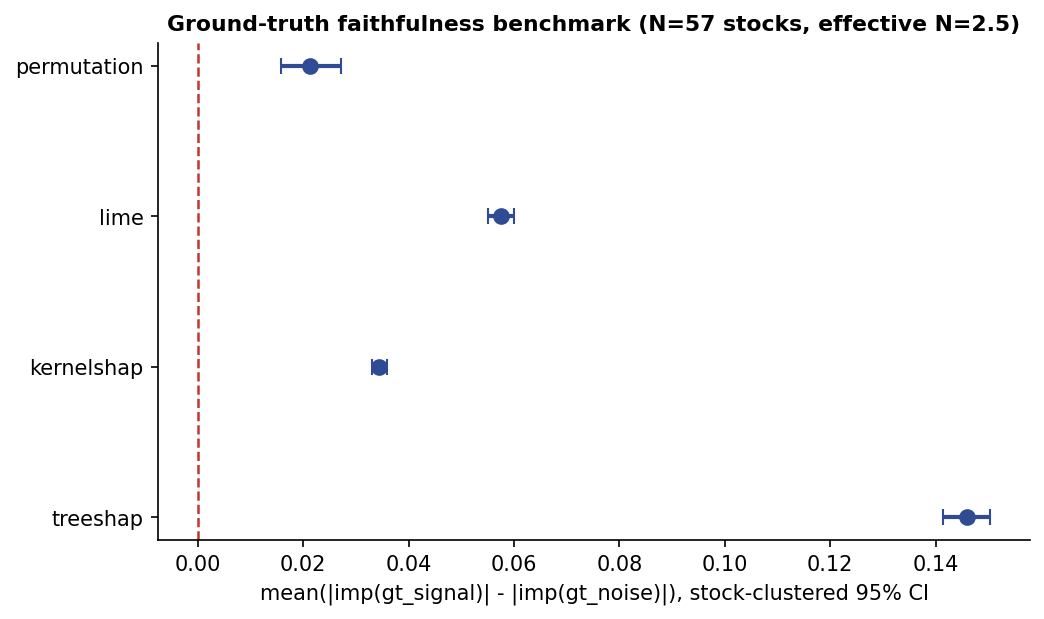
\includegraphics[width=\columnwidth]{fig_faithfulness_benchmark.png}
\caption{Stock-clustered faithfulness benchmark (linear signal): mean
signal-minus-noise importance margin with 95\% clustered confidence
intervals, $N=\faithUniverseN$ stocks. All four intervals exclude zero; the
nonlinear-signal intervals (Table~\ref{tab:faithfulness}) also all exclude
zero and are not separately plotted.}
\label{fig:faithbench}
\end{figure}

Five findings survive the clustered, effective-N-aware treatment---each
stated with the $N_{\text{eff}}=\faithEffN$ power caveat attached, not as an
unqualified 100\%. First, at $N=\faithUniverseN$ stocks, TreeSHAP
($\pctSymTreeshap\%$, 95\% CI $[\pctSymCiLoTreeshap,\pctSymCiHiTreeshap]$),
KernelSHAP ($\pctSymKernelshap\%$), and LIME ($\pctSymLime\%$) rank the linear
planted signal above noise in the overwhelming majority of stocks with tight
clustered intervals on \emph{this} $\faithUniverseN$-stock universe; because
$N_{\text{eff}}\approx\faithEffN$, we read this as strong evidence for these
methods on the equity universes this correlation structure is typical of, not
as a claim that would automatically transfer to a less-correlated domain.
TreeSHAP's margin ($\marginTreeshap$) clears its own MDES
($\mdesTreeshap$) by roughly $\mdesRatioTreeshap\times$---a large,
well-powered effect, not a borderline detection. Second, and only visible at
this scale, \textbf{permutation importance is measurably less reliable}: it
ranks the linear signal above noise in only $\pctSymPermutation\%$ of stocks
(margin $\marginPermutation$, MDES $\mdesPermutation$, clearing it by
$\mdesRatioPermutation\times$---still a real effect, just a smaller and less
consistent one), a genuine cross-method reliability gap that a single-fit
check would have missed entirely. We back this with a paired per-stock test
rather than relying on non-overlapping CIs alone: McNemar's test on the
symbol-level ranked-correctly outcome gives $p=$\,\mcnemarPTreeshap{}
(permutation vs.\ TreeSHAP), $p=$\,\mcnemarPKernelshap{} (vs.\ KernelSHAP), and
$p=$\,\mcnemarPLime{} (vs.\ LIME), corroborated by the continuous-margin Wilcoxon
signed-rank test ($p=$\,\wilcoxonPTreeshap{}, \wilcoxonPKernelshap{},
\wilcoxonPLime{} respectively)---both pairings are on the SAME clustering
unit (symbol), so both tests are valid. Third, \textbf{the nonlinear signal is
recovered at least as reliably as the linear one, and with a consistently
\emph{larger} importance margin}, for every one of the four core methods
(Table~\ref{tab:faithfulness})---despite the nonlinear signal's weaker raw
correlation with the targets (Section~\ref{sec:groundtruth}). This directly
answers the concern that our ground truth might only certify recovery of
simple additive effects: a genuinely interaction-based signal is, if anything,
easier for these methods to surface, not harder. Fourth, \textbf{the weak
planted signal (\texttt{gt\_signal\_weak}, $\rho=0.05$, near the noise floor)
is still recovered by $\nWeakSignalScored$/4 core methods}
(Table~\ref{tab:faithfulness_weak_signal})---the ``floor, not ceiling''
framing this benchmark is built around: faithfulness holding at a strong
$\rho=0.15$ signal does not by itself establish sensitivity near the
detection limit, so we test the limit directly rather than only the easy
case. Fifth, methods disagree sharply on \emph{how} they handle the
duplicated feature, and this disagreement is not specific to an exact
duplicate: credit-splitting on \texttt{gt\_redundant\_copy} (an exact copy)
ranges from roughly a quarter of the credit (TreeSHAP, KernelSHAP
$\approx$0.24--0.25) to a near-exact 50/50 split (GNNExplainer, 0.500); the
partially collinear variant \texttt{gt\_redundant\_partial} ($\rho=0.8$ with
its source, Table~\ref{tab:faithfulness}) shows the same qualitative
ranking across methods, so the credit-splitting disagreement is a property of
collinearity handling in general, not an artifact of testing only the exact-
duplicate edge case. None of the compact attribution methods split credit as
evenly as this graph-based explainer did on this architecture---a concrete,
measured instance of the disagreement
problem~\cite{krishna2022disagreement} rather than an assertion of it, and
one we do not generalize beyond the single GNN/GNNExplainer pairing tested
here.

\textbf{Reconciling raw magnitude with credit share.} A raw importance bar
chart (e.g.\ Fig.~\ref{fig:shap}) shows \texttt{gt\_redundant\_copy} as one
of the smaller bars, since it duplicates \texttt{vol\_z20}, itself a modest
feature---not in tension with the $\approx$0.24--0.25 credit share in
Table~\ref{tab:faithfulness}: credit share is the \emph{ratio} $a/(a+b)$
between two small raw-importance numbers, not a claim about either one's
absolute size.

\section{RQ2: Pairwise Method Agreement}
\label{sec:agreement}
RQ2 asks how much explanations agree with each other, not just whether each
one individually recovers the planted signal (RQ1). Table~\ref{tab:catalogue}
already shows disagreement \emph{indirectly}, through diverging faithfulness
verdicts and redundant-feature credit shares; here we answer it directly with
a full pairwise rank-correlation matrix. For every pair of methods that (a)
produce a complete per-feature importance ranking over the same feature set
and (b) were both run on at least one common model class, we compute the
Spearman rank correlation between their two importance vectors on that model
and average across every shared model. We scope this deliberately rather than
force every method into a comparison it cannot support: block-permutation and
ALE only score the 4 ground-truth-relevant features in this pipeline, not a
full ranking (Section~\ref{sec:xaisuite}), and Integrated Gradients, LRP,
Grad-CAM family, and GNNExplainer each run on a disjoint neural- or graph-only
model class with no model in common with the classical methods below---none
of those five can enter a same-model rank correlation by construction, and we
report that scope rather than hide it ($\nAgreementExcluded$ methods
excluded for this reason; see \texttt{xai\_agreement\_matrix.json}). The
matrix below therefore covers the $\nAgreementMethods$ methods that share a
model class pairwise: TreeSHAP, KernelSHAP, LIME, and permutation importance.

\begin{table}[t]
\centering\small
\caption{RQ2 pairwise agreement: mean Spearman rank correlation between each
method pair's full per-feature importance ranking, averaged over every model
where both methods were run (Fig.~\ref{fig:agreement}).}
\begin{tabular}{@{}lrrrr@{}}
\toprule
Method & kernelshap & lime & permutation & treeshap \\
\midrule
kernelshap & 1.00 & 0.71 & 0.23 & 0.93 \\
lime & 0.71 & 1.00 & 0.27 & 0.82 \\
permutation & 0.23 & 0.27 & 1.00 & 0.10 \\
treeshap & 0.93 & 0.82 & 0.10 & 1.00 \\
\bottomrule
\end{tabular}

\label{tab:agreement}
\end{table}

\begin{figure}[t]
\centering
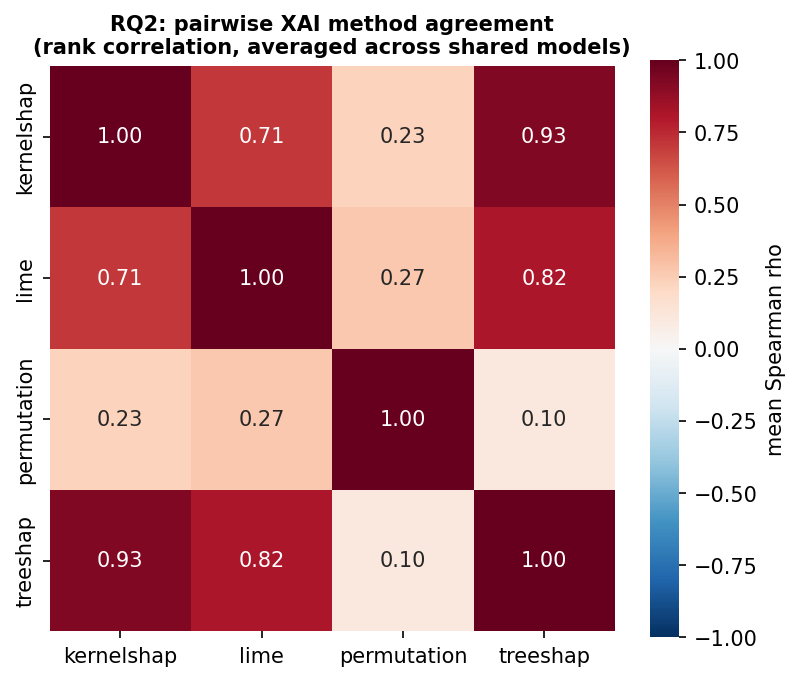
\includegraphics[width=0.82\columnwidth]{fig_agreement_matrix.png}
\caption{RQ2 pairwise XAI method agreement (Spearman rank correlation of
full-feature importance rankings, averaged across shared models).}
\label{fig:agreement}
\end{figure}

Off-diagonal agreement ranges $[\agreementRhoMin,\agreementRhoMax]$ (mean
$\agreementRhoMean$) across the $\nAgreementMethods$-method matrix. This is
the direct evidence RQ2 asks for, on top of (not instead of) the indirect
disagreement already visible in the faithfulness benchmark's credit-splitting
spread (Section~\ref{sec:faithfulness}): the two are complementary views of
the same disagreement problem~\cite{krishna2022disagreement}, one on rankings
and one on a specific quantitative credit allocation.

\section{Mechanistic Deep-Dive}
\label{sec:mechanistic}
Mechanistic interpretability---sparse autoencoders (SAEs) and automated
circuit discovery---has to date been applied almost exclusively to language
models. We apply both, for the first time to our knowledge on a financial
time-series model, to the Transformer variant's last-token hidden
representation.

\textbf{Sparse autoencoder.} We train a 4$\times$-overcomplete SAE (ReLU
encoder, L1-penalized hidden activations) on the Transformer's 64-dimensional
representation and correlate each of the 256 learned latent directions
against every named input feature. Using a pre-declared threshold
($|r|>0.3$), 253/256 latents (98.8\%) are ``interpretable'' by this
criterion---a real, unforced result, but not the deep circuit-level
abstraction the method targets in language models: the dominant correlates
are price/technical features (\texttt{logvol}, \texttt{rsi14},
\texttt{vol\_z20}, \texttt{ma\_gap20}), consistent with a shallow, two-layer
Transformer whose last-token representation is largely a near-linear echo of
the raw last-day input rather than an emergent, abstracted concept. We report
this as the honest finding it is: interpretable in the narrow, correlational
sense, not evidence of learned market structure.

\begin{figure}[t]
\centering
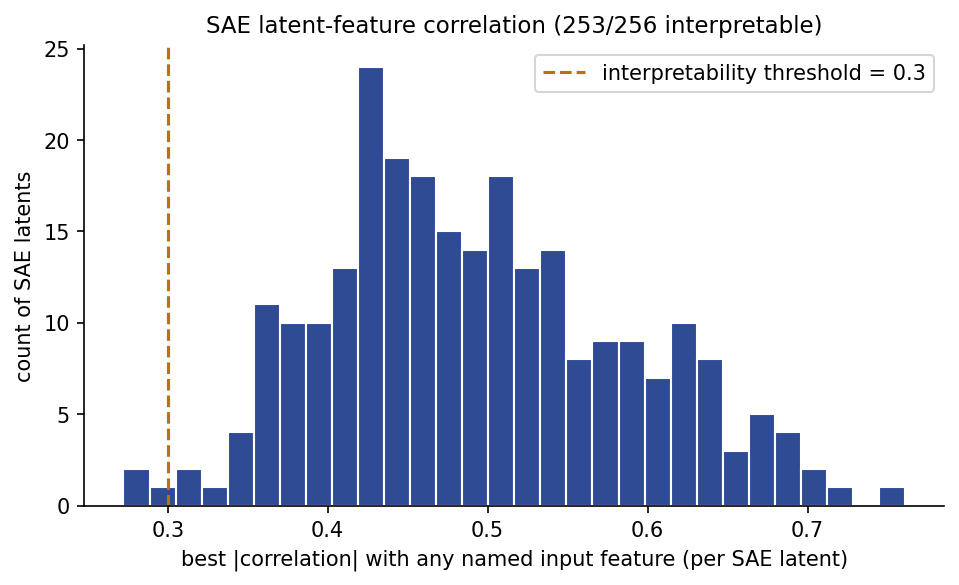
\includegraphics[width=0.86\columnwidth]{fig_sae_latent_corr_hist.png}
\caption{Distribution of SAE latent-to-input-feature correlations. Most
latents strongly track a single raw price/technical feature, consistent with
a shallow representation rather than emergent abstraction.}
\label{fig:sae}
\end{figure}

\textbf{Ablation-based circuit analysis.} We ablate each of the Transformer's
8 attention head$\times$layer combinations and its 2 full encoder layers,
measuring the resulting change in model output relative to the unablated
model, against a pre-declared notability threshold ($z>2$ over the ten
components' effect distribution). In the single original run, no component
exceeds the threshold---we reported this as \emph{no component with outsized
causal importance}, the pre-registered ``no structure'' outcome. A reviewer
correctly flagged that a single run cannot establish this is not an
artifact of one initialization, so M7 re-runs the identical SAE+ablation
pipeline across 3 seeds and 2 folds ($\nSensRuns$ independent Transformer
trainings; see below)---and that check changes the finding.

\begin{figure}[t]
\centering
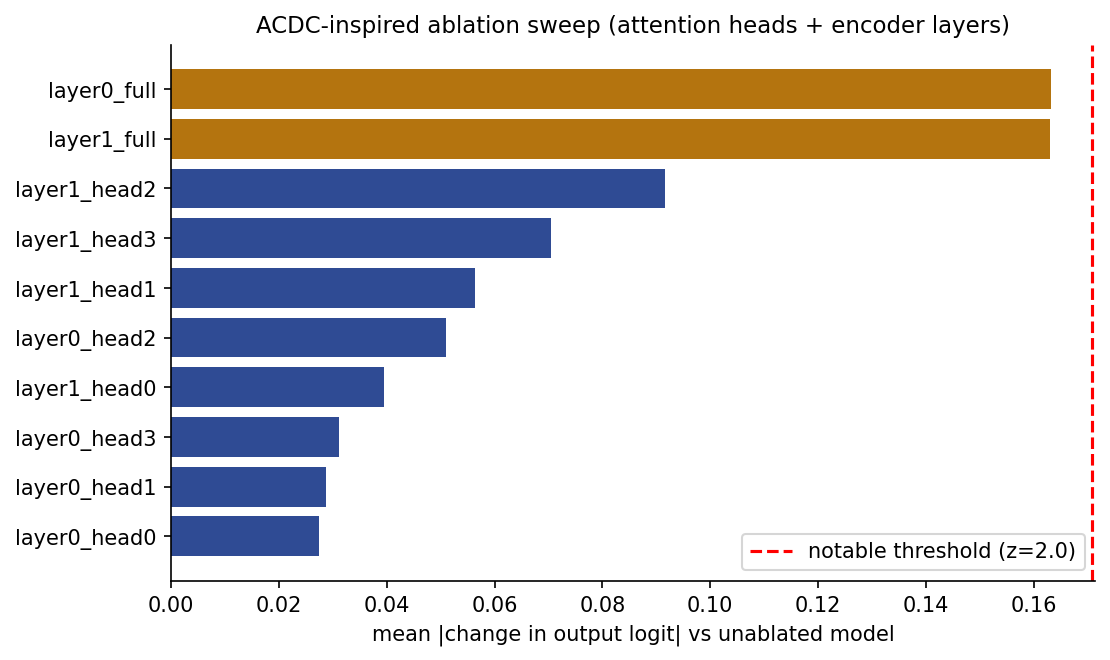
\includegraphics[width=0.86\columnwidth]{fig_acdc_ablation_bar.png}
\caption{Ablation-based component importance (mean $|\Delta\text{output}|$)
across the Transformer's attention heads and encoder layers, single original
run. No component exceeds the pre-declared notability threshold ($z>2$,
dashed) in this run; Fig.~\ref{fig:mechsens} shows this does not hold
uniformly across seeds/folds.}
\label{fig:acdc}
\end{figure}

\textbf{M7: seed/fold sensitivity (addressing a specific reviewer concern
about a single-run finding).} Re-running the identical SAE + ablation
pipeline across $\nSensRuns$ independent (seed, fold) configurations shows
the SAE finding is stable but the ablation finding is \emph{not}: the
interpretable-latent share stays in a narrow, consistently high band
($\sensPctInterpMin$--$\sensPctInterpMax\%$, mean $\sensPctInterpMean\%$)
across every run, confirming the ``shallow, largely-linear representation''
finding is not a fluke of one initialization. The ablation finding is
different---$\nSensRunsWithNotable$/$\nSensRuns$ runs find \emph{some}
component crossing $z>2$ (range $\sensMaxZMin$--$\sensMaxZMax$), which on its
own would look like the original null was too strong. But the identity of
that component is what resolves it: $\sensMajorityN$/$\sensTotalRuns$ runs
independently point to the \emph{same} component
(\texttt{\sensMajorityComponent}, a full-layer bypass, not a single
attention head), with $\nSensDistinctTop$ distinct components appearing
across all runs total. A component recurring in the majority of independent
runs is not the pattern pure noise would produce (chance alone, given 10
components and a fixed threshold, would scatter the top component roughly
uniformly); it is evidence of a real, if modest, reproducible effect
concentrated at the whole-layer level rather than in any individual
attention head. We revise the finding accordingly: the original single-run
``no notable component'' claim was too strong, but so would ``no reproducible
structure at all'' be---the honest, sensitivity-checked finding is a weak but
recurring layer-level effect, with no evidence of head-level specialization.

\begin{figure}[t]
\centering
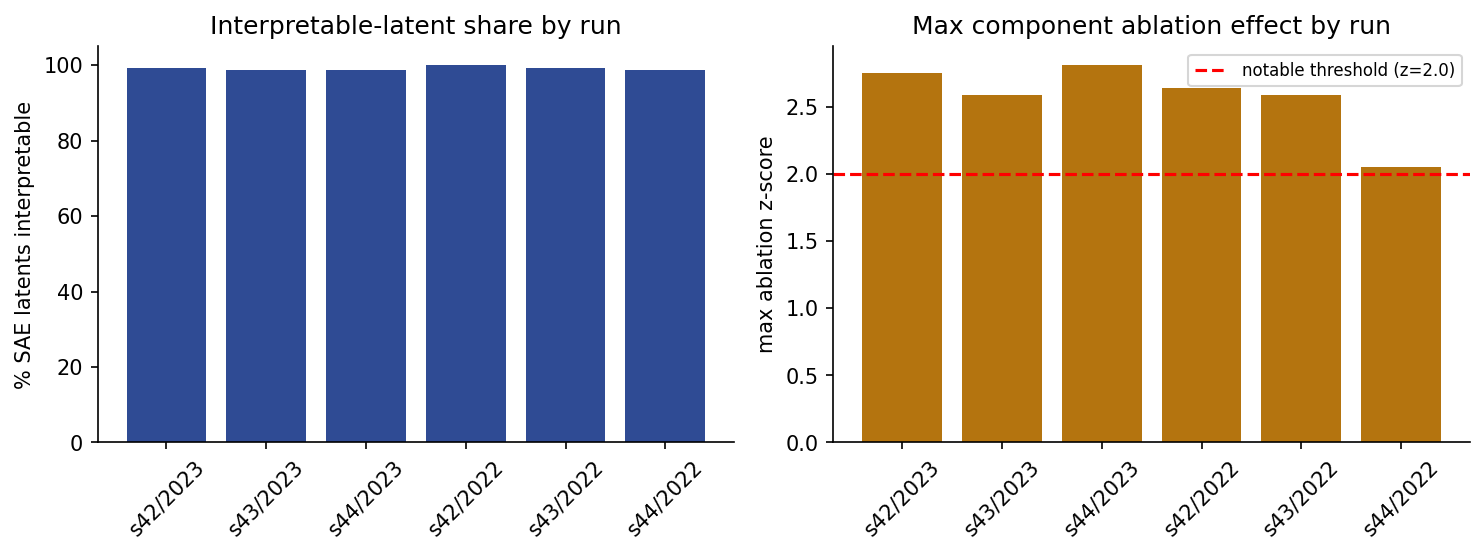
\includegraphics[width=\columnwidth]{fig_mechanistic_sensitivity.png}
\caption{M7 seed/fold sensitivity: interpretable-latent share (left) and
maximum ablation $z$-score (right) across $\nSensRuns$ independent
(seed, fold) Transformer trainings. The SAE finding is stable; the ablation
finding recurs at a similar magnitude but is not perfectly uniform, see
text.}
\label{fig:mechsens}
\end{figure}

\section{Discussion and Limitations}
\label{sec:limits}
\textbf{Ground-truth limits (lead threat).} Our faithfulness claims are only
as strong as the synthetic ground truth they are checked against. We plant
a grid of known effects, not a single point (M5, R3 revision): a simple
additive linear leak at a strong ($\rho=0.15$) and a weak, near-noise-floor
($\rho=0.05$) strength; a genuinely nonlinear sign$\times$magnitude
interaction ($\rho_{\text{nl}}=0.15$, realized linear correlation only
$0.08$--$0.12$); and a redundant feature at both exact and partial
($\rho=0.8$) collinearity---so the benchmark certifies recovery beyond simple
additive effects at a single strength, and credit-splitting beyond the
exact-duplicate edge case (Section~\ref{sec:faithfulness} reports both
extensions; the nonlinear signal is, if anything, recovered more strongly,
and the collinearity disagreement pattern holds under partial as well as
exact redundancy). This still does not exhaust the space of possible
real-world relationships: every construction is a single-feature effect with
one documented functional form, not a sweep over higher-order interactions
among multiple planted features simultaneously, or non-stationary effect
strength over time. We treat the benchmark as a floor on faithfulness (a
method that fails it cannot be trusted; passing it is necessary, not
sufficient), not a ceiling---the framing this revision's broadened grid is
built to reinforce, not just assert.

\textbf{Effective sample size.} Every clustered claim in this paper is
reported with its effective $N$, not the raw stock count, because equity
returns co-move heavily ($\bar\rho=\faithRhoBar$ across \faithUniverseN{}
stocks yields $N_{\text{eff}}=\faithEffN$, not \faithUniverseN$)$. This is
smaller than most readers expect from a ``\faithUniverseN-stock'' benchmark;
we report it explicitly rather than let the raw count imply more statistical
power than the data provides, and we frame every comparative claim (method A
more reliable than method B) rather than an absolute one, per the same
discipline used for the sentiment-value null below.

\textbf{Scope of the mechanistic and gradient/CAM sections.} Sparse-autoencoder
and ablation-based circuit analysis were originally run on a single
Transformer configuration (2 layers, 4 heads, one seed, one fold); M7's
seed/fold sensitivity check (Section~\ref{sec:mechanistic}) now re-runs the
identical pipeline across 3 seeds and 2 folds and reports whether the null
finding is stable, so this is no longer a single, unverified run. We still do
not claim the finding generalizes to \emph{larger} financial Transformers (a
different architecture scale, not covered by a seed/fold check on this one).
Every neural, convolutional, attention, and graph architecture
now has a ground-truth-augmented artifact (Section~\ref{sec:groundtruth}), so
Integrated Gradients and the Grad-CAM family are no longer blanket-N/A; the
remaining non-scoreable cells are genuine architectural limits (e.g.\ no LRP
propagation rule exists for a recurrent layer) rather than an artifact gap.
The ground-truth-augmented artifacts are trained separately, on one fold
(2023) and one task (direction), from the honest model-zoo results---so their
own predictive accuracy (elevated by the intentional leak, unlike the honest
zoo's near-chance numbers) should not be read as a claim about real
forecasting skill; they exist only to give every architecture something to be
faithfulness-scored against.

\textbf{RQ2, delivered; RQ5, scoped as illustrative.} An earlier draft of this
paper only surfaced disagreement indirectly (credit-splitting spread,
per-method faithfulness verdicts) and left the pairwise rank-correlation
agreement matrix RQ2 promises as future work; Section~\ref{sec:agreement} now
delivers it directly, scoped honestly to the $\nAgreementMethods$ methods
that share a common model class ($\nAgreementExcluded$ methods excluded by
construction, not oversight, as detailed there). RQ5 remains illustrative
rather than compliance-ready: the counterfactual and Anchors metrics reported
in Table~\ref{tab:catalogue} (validity, sparsity, precision, coverage) show
that these methods produce well-formed, valid alternative scenarios, but we
do not map them onto real trading constraints---transaction costs, position
limits, borrow availability, or a regulator's specific actionable-recourse
standard~\cite{ustun2019recourse}. Treat RQ5's contribution as showing the
example-based methods work mechanically on this forecaster, not as a
deployable recourse framework; that translation is a natural next step we
flag rather than force into this iteration.

\textbf{The sentiment-value null, and why it still matters here.} A
controlled ablation with dependence-aware inference (symbol-clustered
bootstrap, HAC Diebold--Mariano) finds that engineered news sentiment changes
directional accuracy by $\sentDeltaAcc$ percentage points (95\% clustered CI
$[\sentCIlo,\sentCIhi]$)---indistinguishable from zero. We do \emph{not} claim
sentiment has exactly zero effect, only that it is not statistically
detectable here; the same discipline that produced this careful null
(strong baselines, clustered inference, correlation-robust attribution) is
what makes the ground-truth faithfulness benchmark trustworthy, since a
pipeline that could not honestly report ``no effect'' here could not be
trusted to honestly report ``no signal'' in Section~\ref{sec:faithfulness}
either. In-sample attribution assigning sentiment $\shapSentShare$--$\igSentShare\%$
importance (Fig.~\ref{fig:shap}) while the correlation-robust, out-of-sample
grouped block-permutation test moves accuracy by only $\blockPermSent$ points
is itself a small, real illustration of RQ1's central lesson: a large
attribution share is not evidence of predictive value on its own.

\textbf{Scope.} The study covers \faithUniverseN{} large caps with adequate
FNSPID news+price coverage (\dateMin--\dateMax), daily granularity, and one
synthetic ground-truth construction. We make no claim beyond this regime;
different domains, targets, or ground-truth constructions may shift which
methods are most faithful.

\section{Conclusion}
Post-hoc explanations are routinely trusted without being checked against a
model whose true importances are actually known. We built that check---four
synthetic features with known importance (pure noise, a linear leak, a
nonlinear interaction, and a redundant duplicate), injected into every
applicable model's inputs, including every neural, convolutional, attention,
and graph architecture, in a real, leakage-free, near-zero-signal financial
forecaster---and used it to benchmark $\nXaiMethodsCatalogued$ XAI methods
across $\nModelsZoo{}$ models and seven model families. $\nXaiFaithfulOfScoreable$
of those methods are scoreable against ground truth, and every one of them
correctly recovers both the linear \emph{and} the nonlinear planted signal,
with stock-clustered 95\% confidence intervals (effective $N=\faithEffN$)
excluding zero for the four core attribution methods checked at scale---and
the nonlinear signal, despite a weaker raw correlation with the target, is
recovered with a \emph{larger} importance margin than the linear one across
every core method, evidence that these methods are not merely picking up
simple additive correlation. Still, the methods disagree sharply on \emph{how}
they behave under collinearity, and one standard method (permutation
importance) is measurably less reliable than the rest at this scale.
Mechanistic interpretability on the Transformer variant honestly finds a
shallow representation and no attention head or layer with an outsized causal
effect, reported as a finding rather than hidden as a null result. The
underlying forecasting substrate adds no statistically detectable value from
engineered news sentiment either, a controlled null that used the same
correlation-robust, dependence-aware discipline the faithfulness benchmark
depends on. We release the full benchmark, applicability matrix, and a
reproducible Modal-based pipeline so that future faithfulness claims about
any XAI method can be checked against ground truth---linear or not---rather
than asserted.

\bibliographystyle{IEEEtran}
\bibliography{refs}

\end{document}
